% =============================================================================
% THE INCOHERENCE
% Author: Flyxion
% Engine: LuaLaTeX (required — do not use pdfLaTeX or XeLaTeX)
% Compile: lualatex main.tex  (run twice for cross-references)
%
% FONT REQUIREMENTS — place all files in ./fonts/
%   NovaMonoStandardGalactic.ttf    Sga-Regular.ttf
%   CursiveGalactic-Regular.ttf     Amiri-Regular.ttf
%   Amiri-Bold.ttf                  Amiri-Italic.ttf
%   Amiri-BoldItalic.ttf            Cheiro-Regular.ttf
%   Clypto-Regular.ttf              Logico_philosophicus-Regular.ttf
%   Systada-Regular.ttf             Lingojam_cipher-Regular.ttf
%   dactyl.ttf                      shapeform.ttf
% =============================================================================

\documentclass[12pt,twoside,openany]{book}

\usepackage{fontspec}
\usepackage{unicode-math}

\usepackage[
  a4paper,
  top=2.5cm, bottom=3.0cm,
  inner=2.8cm, outer=2.2cm,
  twoside
]{geometry}

\usepackage{polyglossia}
\setdefaultlanguage{english}
\setotherlanguage{arabic}

\newcommand{\fontdir}{fonts/}

% --- Primary font regimes ---
\setmainfont{NovaMonoStandardGalactic.ttf}[Path=\fontdir, Scale=1.0]
\newfontfamily\SGA{Sga-Regular.ttf}[Path=\fontdir, Scale=1.05]
\newfontfamily\CursiveSGA{CursiveGalactic-Regular.ttf}[Path=\fontdir, Scale=1.05]
\newfontfamily\AmiriFont{Amiri-Regular.ttf}[Path=\fontdir, Script=Arabic, Scale=1.15]
\newfontfamily\arabicfont{Amiri-Regular.ttf}[Path=\fontdir, Script=Arabic, Scale=1.15]

% --- Derived font regimes ---
\newfontfamily\Logico{Logico_philosophicus-Regular.ttf}[Path=\fontdir, Scale=1.0]
\newfontfamily\Cheiro{Cheiro-Regular.ttf}[Path=\fontdir, Scale=1.0]
\newfontfamily\Clypto{Clypto-Regular.ttf}[Path=\fontdir, Scale=1.0]
\newfontfamily\Systada{Systada-Regular.ttf}[Path=\fontdir, Scale=1.0]
\newfontfamily\Dactyl{dactyl.ttf}[Path=\fontdir, Scale=1.0]
\newfontfamily\Shapeform{shapeform.ttf}[Path=\fontdir, Scale=1.0]

% --- Inline switching macros ---
\newcommand{\sga}[1]{{\SGA #1}}
\newcommand{\cga}[1]{{\CursiveSGA #1}}
\newcommand{\logico}[1]{{\Logico #1}}
\newcommand{\cheiro}[1]{{\Cheiro #1}}
\newcommand{\clypto}[1]{{\Clypto #1}}
\newcommand{\sys}[1]{{\Systada #1}}

% --- Arabic block environment ---
\newenvironment{AR}{\begin{arabic}}{\end{arabic}}

% --- Typography packages ---
\usepackage{microtype}
\usepackage{setspace}
\usepackage{ragged2e}
\usepackage{calc}

% --- Layout packages ---
\usepackage{multicol}
\usepackage{paracol}
\usepackage{marginnote}
\usepackage{changepage}
\usepackage{afterpage}
\usepackage{atbegshi}

% --- Spatial packages ---
\usepackage{tikz}
\usetikzlibrary{calc,positioning}
\usepackage{rotating}
\usepackage{graphicx}

% TikZ positioned text (for drift effects)
\newcommand{\drifttext}[3]{%
  \begin{tikzpicture}[remember picture,overlay]
    \node at ($(current page.center)+(#1,#2)$) {#3};
  \end{tikzpicture}%
}
\newcommand{\rotblock}[1]{\rotatebox{180}{#1}}
\newcommand{\tiltblock}[2]{\rotatebox{#1}{#2}}

% =============================================================================
% DUAL PAGINATION SYSTEM
%
% Left margin (outer):  Western Arabic-numeral page numbers
% Right margin (inner): Eastern Arabic-script numerals via Amiri
%
% Read direction: outside-in on both sides.
%
% BYOBU DRIFT CYCLE (chapters XII-XIV then XV-XVII):
%   Drift:  right pages step Arabic counter TWICE → Arabic runs ahead
%           Arabic numerals rendered in Dactyl font
%   Return: left pages hold Arabic counter → English catches up
%           Western numerals rendered in Dactyl font
%   One cycle only. No announcement.
% =============================================================================

\usepackage{fancyhdr}

\newcounter{arabicpagectr}
\setcounter{arabicpagectr}{0}

% Eastern Arabic numeral rendering via polyglossia
\newcommand{\arabicpagenum}{%
  {\AmiriFont\arabicnumerals{\value{arabicpagectr}}}%
}

\newcommand{\stepArabicPage}{\stepcounter{arabicpagectr}}

% Normal synchronized pagestyle
\fancypagestyle{incoherence}{%
  \fancyhf{}
  \fancyfoot[LE]{\small\thepage}
  \fancyfoot[RO]{\small\thepage}
  \fancyfoot[RE]{\small\arabicpagenum}
  \fancyfoot[LO]{\small\arabicpagenum}
  \renewcommand{\headrulewidth}{0pt}
  \renewcommand{\footrulewidth}{0pt}
}

% Byobu drift: Arabic runs ahead, rendered in Dactyl
\fancypagestyle{byobu-drift}{%
  \fancyhf{}
  \fancyfoot[LE]{\small\thepage}
  \fancyfoot[RO]{\small\thepage}
  \fancyfoot[RE]{{\Dactyl\arabicpagenum}}
  \fancyfoot[LO]{{\Dactyl\arabicpagenum}}
  \renewcommand{\headrulewidth}{0pt}
  \renewcommand{\footrulewidth}{0pt}
}

% Byobu return: Western numerals in Dactyl, English catching up
\fancypagestyle{byobu-return}{%
  \fancyhf{}
  \fancyfoot[LE]{{\Dactyl\thepage}}
  \fancyfoot[RO]{{\Dactyl\thepage}}
  \fancyfoot[RE]{\small\arabicpagenum}
  \fancyfoot[LO]{\small\arabicpagenum}
  \renewcommand{\headrulewidth}{0pt}
  \renewcommand{\footrulewidth}{0pt}
}

% Empty pagestyle for high-fragmentation chapters
\fancypagestyle{incoherence-empty}{%
  \fancyhf{}
  \renewcommand{\headrulewidth}{0pt}
}

\pagestyle{incoherence}

% Byobu mechanics
% Right-page split: Arabic counter steps twice (drift phase)
\newcommand{\rightpagesplit}{%
  \stepArabicPage%
  \stepArabicPage%
}
% Left-page catch: Arabic counter NOT stepped; English advances via \thepage
\newcommand{\leftpagecatch}{}

% =============================================================================
% GLOBAL STYLE
% =============================================================================

\setstretch{1.05}
\setlength{\parindent}{0pt}
\setlength{\parskip}{0.4em}

\usepackage{titlesec}
\titleformat{\chapter}[block]{\normalfont\normalsize}{}{0pt}{}
\titlespacing*{\chapter}{0pt}{2em}{1.5em}
\titleformat{\section}[block]{\normalfont\small}{}{0pt}{}
\titlespacing*{\section}{0pt}{1.5em}{1em}

% =============================================================================
% DOCUMENT BODY
% =============================================================================

\begin{document}

\setcounter{arabicpagectr}{1}

% --------------------------------------------------------------------------
% FRONT MATTER
% --------------------------------------------------------------------------

\pagestyle{incoherence-empty}

\begin{titlepage}
\vspace*{6cm}
\begin{center}
{\large\sga{THE INCOHERENCE}}

\vspace{1.5em}

{\normalsize Flyxion}

\vspace{1em}

{\small Independent Researcher}

\vspace{3em}

{\footnotesize\textit{Based on the life and work of
Ibn Rushd (Averroes, 1126--1198)}}
\end{center}
\end{titlepage}

\cleardoublepage

% Epigraph
\thispagestyle{incoherence-empty}
\vspace*{8cm}
\begin{flushright}
\begin{minipage}{0.6\textwidth}
\begin{AR}
التهافت والتهافت
\end{AR}

\vspace{1em}

\cga{The incoherence of the incoherence.}

\vspace{1em}

\sga{What binds the world does not explain itself.}
\end{minipage}
\end{flushright}

\cleardoublepage
\pagestyle{incoherence}

% ==========================================================================
% PART ONE — STABLE SYSTEM
% Chapters: scenery intercalation, I, II
% Typography: Nova Mono dominant, first SGA anomaly (Chapter I only)
% ==========================================================================

\stepArabicPage
% =============================================================================
% INTERCALATIO: DE LOCO ET REBUS
% Status: DRAFTED — early insertion chapter
% Placement: Before Chapter III (before instability begins)
% Pure scenery. Minimal instability — single SGA mark, unremarked.
% Establishes pre-narrative ontology. Teaches reader how to read.
% =============================================================================

\chapter*{Intercalatio: De Loco et Rebus}
\addcontentsline{toc}{chapter}{De Loco et Rebus}

\setstretch{1.05}

\begin{adjustwidth}{2.4cm}{2.4cm}

The courtyard is rectangular.

\vspace{1em}

Stone defines it.

\vspace{2em}

\end{adjustwidth}

\begin{adjustwidth}{3.0cm}{2.0cm}

The ground is paved in alternating slabs, light and dark, not perfectly aligned,
but consistent enough to be taken as intention.

\vspace{1em}

Water runs through a narrow channel cut into the center.

\vspace{1em}

It moves slowly.

\vspace{2em}

\end{adjustwidth}

\begin{adjustwidth}{2.8cm}{2.2cm}

A basin interrupts the channel.

\vspace{1em}

Circular. Shallow. The surface reflects only what is directly above it.

\vspace{2em}

\end{adjustwidth}

\begin{adjustwidth}{3.2cm}{2.0cm}

Along the edges: columns, evenly spaced, not identical. Their bases worn
differently. Their capitals intact.

\vspace{2em}

\end{adjustwidth}

\begin{adjustwidth}{2.6cm}{2.6cm}

Between the columns: air. Light. Dust suspended.

\vspace{2em}

\end{adjustwidth}

\begin{adjustwidth}{3.4cm}{2.0cm}

The walls hold markings. Not all are legible. Some are shallow, as if traced
once and abandoned. Some are deeper, repeated until the surface gave way.

\vspace{1em}

One mark appears again:

\vspace{1em}

\sga{𐌍}

\vspace{1em}

It is not emphasized.

\vspace{2em}

\end{adjustwidth}

\begin{adjustwidth}{2.8cm}{2.2cm}

A door is set into the far wall. Wood. Reinforced. Closed.

\vspace{2em}

The handle shows use. The hinges do not. The threshold is worn.

\vspace{2em}

\end{adjustwidth}

\begin{adjustwidth}{2.6cm}{2.6cm}

Above: open sky. No obstruction. Light entering without interruption.

\vspace{2em}

\end{adjustwidth}

\begin{adjustwidth}{3.0cm}{2.0cm}

A sound is present.

\vspace{1em}

Not continuous. Not absent.

\vspace{2em}

\end{adjustwidth}

\begin{center}
Drip
\end{center}

\begin{adjustwidth}{2.6cm}{2.6cm}

The source is not immediately visible. It is not concealed.

\vspace{2em}

\end{adjustwidth}

\begin{adjustwidth}{3.4cm}{2.0cm}

In the corner: a vessel, empty or nearly empty. Its interior marked by a
line indicating a previous level.

\vspace{2em}

A second vessel nearby. Not aligned. Closer to the wall. Unmarked.

\vspace{2em}

\end{adjustwidth}

\begin{adjustwidth}{3.2cm}{2.0cm}

The difference is small.

\vspace{1em}

It remains.

\vspace{2em}

\end{adjustwidth}

\begin{adjustwidth}{2.6cm}{2.6cm}

No one enters.

\vspace{1em}

No one leaves.

\vspace{2em}

\end{adjustwidth}

\begin{adjustwidth}{3.0cm}{2.0cm}

The arrangement persists. Not perfectly. Sufficiently.

\vspace{2em}

\end{adjustwidth}

\begin{center}
Drip
\end{center}

\begin{adjustwidth}{2.6cm}{2.6cm}

Nothing is explained.

\vspace{1em}

Nothing requires explanation.

\vspace{2em}

\end{adjustwidth}


\stepArabicPage
% =============================================================================
% INCOHERENTIA I: DE PULSU ET CAUSA
% Status: DRAFTED
% Typographic state: Nova Mono dominant. Single SGA anomaly (\sga{cause}).
% System fully stable. The anomaly is unannounced and unrepeated.
% The drip enters without emphasis.
% =============================================================================

\chapter*{Incoherentia I: De Pulsu et Causa}
\addcontentsline{toc}{chapter}{I. De Pulsu et Causa}

\setstretch{1.05}

Midday in Córdoba. The light falls not gently but with incision, dividing
the courtyard into regions of clarity and remainder. Limestone returns the
sun without mercy. Edges declare themselves. Surfaces admit no ambiguity.

Beneath a stretched canvas awning there is arranged a table of modest
dimension yet exact proportion. Upon it are laid instruments not in ornament
but in sequence: brass, linen, ceramic, water. Each object occupies a place
that is neither arbitrary nor explained. The order is sufficient.

Averroes sits cross-legged. The posture is not affectation but economy. His
hands bear the record of repetition: ink embedded in the folds, faint scars
crossing the knuckles where blade has met resistance. He does not display
them. They are already known.

Before him, a man of labor. The shoulder is swollen, the skin drawn taut
and bright with heat. The body speaks in gradients.

Around them, students in a semicircle. Their arrangement is not symmetrical,
yet it resolves into balance. They lean forward not in unison but in
convergence.

At the rear, a figure remains still. Hood drawn. Presence withheld rather
than concealed.

Averroes takes the patient's wrist. Thumb and forefinger find the pulse
without search. His eyes close, not in contemplation but in subtraction.

There is no sound of the pulse. Yet the air acquires a rhythm, faintly,
as though breath itself had been persuaded into measure.

He releases the wrist.

He does not immediately look at the wound.

He looks instead to the basin of water. Then to the angle of shadow cast
along the wall. Time is read indirectly, as one reads the consequence rather
than the declaration.

\medskip

\textbf{AVERROES}

The pulse is fast but regular. The heat is localized. The skin is red, not
darkened. This tells us the body is reacting, not failing.

\medskip

A student leans forward. The question arrives already sharpened.

\medskip

\textbf{STUDENT}

Master, how can we be certain this reaction is the \sga{cause}, and not
merely the sign?

\medskip

Averroes turns. Slowly. Not to correct, but to preserve the question from
collapse.

\medskip

\textbf{AVERROES}

Because signs repeat. Causes persist. If you confuse them, you will chase
shadows until the patient dies of patience.

\medskip

A murmur, restrained. Some assent, some hesitation. The distinction has not
yet settled.

\medskip

\textbf{STUDENT}

But some say illness is a test. That the body suffers because God wishes
it so.

\medskip

The statement does not disrupt the circle. It diffuses through it, finding
places to rest.

Averroes adjusts his grip on the lancet. Not defensive. Grounding.

\medskip

\textbf{AVERROES}

If you believe that, you may pray. Prayer is not forbidden here.

\medskip

A pause. Not rhetorical. Functional.

\medskip

\textbf{AVERROES}

But if you stay, you will observe first. Intention does not substitute for
attention.

\medskip

He raises the lancet. The blade receives the light and returns it without
distortion.

\medskip

\textbf{AVERROES}

This tool has no theology. It cuts whether you are righteous or cruel. That
is not blasphemy. That is reliability.

\medskip

The incision is small. Exact. The patient flinches, then exhales as pressure
releases. Fluid emerges, dark, edged with amber. It collects without urgency.

The courtyard contracts, then resumes.

Averroes cleans the wound. The gesture is continuous, unbroken by commentary.

At the edge of the courtyard, in shadow, a vessel releases water into
another. Drop by drop. No emphasis is given. No explanation offered.

The sound is present.

\medskip

\textbf{AVERROES}

When you see suffering, do not ask first what God intends. Ask what the body
is doing. Healing leaves traces. So does decay.

\medskip

A beat.

\medskip

\textbf{AVERROES}

If you refuse to read those traces, you will call ignorance piety and
negligence humility.

\medskip

The binding is applied. Firm, but not excessive.

The patient nods. Gratitude expressed without words.

Students disperse, slowly, carrying fragments of the demonstration with them.
Not all fragments are compatible.

The hooded figure remains.

Averroes packs his instruments. Each returned to its place, though no place
has been declared.

He pauses.

Not turning.

Acknowledgment withheld, or deferred.

\medskip

The vessel continues its work.

\medskip

Drip.

\medskip

Drip.

\medskip

Drip.


\stepArabicPage
% =============================================================================
% INCOHERENTIA II: DE LEGE ET NEGLIGENTIA
% Status: DRAFTED
% Typographic state: SGA clusters around juridical terms: fault, necessity,
% consistency, causes, negligence, excuses. Nova Mono still dominant surface.
% Cursive Galactic absent — that absence is now meaningful.
% The drip returns, louder. No longer ignorable.
% =============================================================================

\chapter*{Incoherentia II: De Lege et Negligentia}
\addcontentsline{toc}{chapter}{II. De Lege et Negligentia}

\setstretch{1.05}

The light that enters the hall is the same light as in the courtyard, yet it
arrives disciplined. It is filtered through lattice and divided into geometry.
What was previously direct is now mediated.

The air is cooler. Not by accident, but by construction.

Bodies are arranged in rows, each posture calibrated to signal attention
without intimacy. Scrolls are present, but unopened. Authority resides not
in reading, but in the possibility of reference.

At the center, elevated without ostentation, sits Averroes.

The instruments have changed. The hands have not.

Before him stand two men. Between them, an absence: a wall that once held.

\medskip

\textbf{JUNIOR JURIST}

The matter before the court concerns injury sustained during the collapse of
a retaining wall on the eastern works. The question is whether \sga{fault}
may be assigned.

\medskip

The word does not settle easily. It remains suspended, as though awaiting a
structure capable of receiving it.

\medskip

\textbf{AVERROES}

Let the builder speak.

\medskip

The builder does not look at the injured man. His gaze fixes just above the
assembly, as if addressing a height that might absolve him.

\medskip

\textbf{BUILDER}

The wall stood as walls stand. Stone upon stone. Mortar mixed as my father
taught me. It fell because God willed it to fall.

\medskip

A murmur. Not resistance. Relief.

The statement requires no verification.

\medskip

\textbf{BUILDER}

Who am I to argue with the decree of the Most High?

\medskip

The laborer shifts. Pain is visible, but not yet admissible.

\medskip

\textbf{LABORER}

I was beneath it, my lord. I heard a crack before it fell. Like dry wood.

\medskip

The builder's jaw tightens.

\medskip

\textbf{BUILDER}

Stone cracks when God commands it.

\medskip

Averroes lowers his eyes. The stylus marks the tablet. The motion is small,
but not negligible.

\medskip

\textbf{AVERROES}

How long had the wall stood?

\medskip

\textbf{BUILDER}

Two seasons. Nearly three.

\medskip

\textbf{AVERROES}

And the mortar?

\medskip

\textbf{BUILDER}

Lime and sand. As always.

\medskip

\textbf{AVERROES}

From which quarry came the stone?

\medskip

The hesitation is brief. It is sufficient.

\medskip

\textbf{BUILDER}

The northern cut. Cheaper transport.

\medskip

Averroes looks up. Not accusing. Locating.

\medskip

\textbf{AVERROES}

The northern stone fractures along internal seams when improperly cured. It
demands thicker mortar and longer setting time.

\medskip

The room tightens. A structure begins to form.

\medskip

\textbf{JUNIOR JURIST}

Qadi, if I may---does this not presume that the wall obeys \sga{necessity}
rather than divine immediacy?

\medskip

The question does not seek answer alone. It seeks boundary.

Averroes does not respond immediately. He looks instead at the laborer's arm.

\medskip

\textbf{AVERROES}

If I said the arm broke because God willed it, would you refuse the splint?

\medskip

Unease enters. It does not dissipate.

\medskip

\textbf{JUNIOR JURIST}

No, my lord, but---

\medskip

\textbf{AVERROES}

Then you already believe that God's will includes \sga{consistency}.

\medskip

A pause. Longer than required.

\medskip

\textbf{AVERROES}

Law cannot function if injury is inscrutable. If every collapse is miracle,
then no craft exists---only luck and prayer.

\medskip

He turns to the builder.

\medskip

\textbf{AVERROES}

You chose cheaper stone. You reduced mortar. You hurried the setting. These
are \sga{causes}.

\medskip

The word does not dissolve.

\medskip

\textbf{AVERROES}

God did not conceal them from you.

\medskip

The builder bows. The motion is correct. The interior is not.

\medskip

Averroes writes.

\medskip

\textbf{AVERROES}

Judgment: \sga{negligence}.

Compensation is owed. The injured man will receive wages for the season lost,
paid by the builder's guild.

\medskip

The stylus presses more firmly than before.

The word remains.

\medskip

The laborer exhales. Relief and disbelief coexist without resolving.

The builder withdraws. Containment replaces defense.

\medskip

The court prepares to proceed. Continuity reasserts itself.

Yet something has been introduced that does not return to prior state.

\medskip

\textbf{JUNIOR JURIST}

Qadi\ldots\ some will say that this ruling limits God.

\medskip

Averroes looks at him. Not as superior, but as instrument.

\medskip

\textbf{AVERROES}

No.

\medskip

A pause.

\medskip

\textbf{AVERROES}

It limits \sga{excuses}.

\medskip

Silence. Not absence of sound, but suspension of interpretation.

\medskip

At the side wall, recessed in stone, a vessel continues its work.

The same rhythm as before.

Yet now it is no longer ignorable.

\medskip

Drip.

\medskip

Drip.

\medskip

Drip.


% ==========================================================================
% PART TWO — BIFURCATION
% Chapters III–VIII
% Cursive SGA enters; Arabic enters; spatial fragmentation begins;
% SGA propagates into connective tissue; drip desynchronizes
% ==========================================================================

\stepArabicPage
% =============================================================================
% INCOHERENTIA III: DE VOCE ET FLUMINE
% Status: DRAFTED
% Typographic state: Cursive Galactic enters for the first time, in the
% preacher's rhetoric. Arabic enters as non-translated expansion layer.
% Nova Mono no longer uncontested. System no longer closed.
% Drip returns distributed, not localized. Not synchronized with itself.
% =============================================================================

\chapter*{Incoherentia III: De Voce et Flumine}
\addcontentsline{toc}{chapter}{III. De Voce et Flumine}

\setstretch{1.05}

The street does not admit geometry.

Where the court imposed alignment, the market dissolves it. Movement replaces
arrangement. Sound replaces structure. The air is no longer divided but
saturated.

Vendors speak across one another without conflict. Calls overlap, not as
argument but as accumulation. Meaning does not reside in sequence, but in
density.

Averroes walks without escort. His pace is neither hurried nor slow. It
adjusts, continuously, to the flows it encounters.

The smell of spice, leather, heat, and dust forms a composite that resists
separation.

At the far end of the street, a voice rises.

Not louder than the others.

But it does not dissipate.

\medskip

\textbf{PREACHER}

\cga{You measure what cannot be contained. You weigh what was never given
weight. You draw lines through water and call them law.}

\medskip

Some turn. Not all.

The voice continues, uninterrupted by the lack of universal attention.

\medskip

\textbf{PREACHER}

\cga{God is not bound by your sequences. He is not contained in your causes.
He does not repeat so that you may learn Him.}

\medskip

Averroes does not stop.

But his trajectory bends.

\medskip

\textbf{PREACHER}

\cga{You say: this leads to that. You say: this must follow. You say: the
world is held together by necessity.}

\medskip

The word emerges again, but it does not stabilize the line.

\medskip

\textbf{PREACHER}

\cga{There is no \sga{necessity}. There is only will. Renewed at every
instant. Destroyed at every instant.}

\medskip

A small crowd gathers. Not in formation. In attraction.

\medskip

\begin{AR}
الحمد لله الذي لا تُقاس أفعاله، ولا تُحدّ مشيئته، ولا تُربط قدرته بسببٍ ولا بعلة.
\end{AR}

\medskip

The Arabic does not translate. It expands.

\medskip

\textbf{PREACHER}

\cga{You seek certainty because you fear interruption. You build systems
because you cannot endure that the world may not return to you as you
expect.}

\medskip

A man laughs. Not in mockery. In recognition.

\medskip

\textbf{PREACHER}

\cga{But what if it does not return? What if the fire does not burn? What if
the blade does not cut? What if the wall stands one day and falls the next
without reason?}

\medskip

The words do not resolve into argument. They circulate.

Averroes stops.

Not at the center. Slightly to the side.

\medskip

\textbf{AVERROES}

If the blade does not cut, then it is no longer a blade.

\medskip

The preacher turns.

The space between them does not close.

\medskip

\textbf{PREACHER}

\cga{Or perhaps it cuts only when commanded.}

\medskip

\textbf{AVERROES}

Then no command could be trusted. Not even yours.

\medskip

A pause.

The crowd leans without moving.

\medskip

\textbf{PREACHER}

\cga{Trust is not given to the world. It is given to God.}

\medskip

\textbf{AVERROES}

And yet you speak to men.

\medskip

The preacher smiles. Not concession. Not victory.

Continuation.

\medskip

\textbf{PREACHER}

\cga{Because they listen.}

\medskip

The answer does not close the exchange. It redirects it into a space without
boundary.

\medskip

\begin{AR}
بل لأن القلوب تميل، لا لأن العقول تُقنع.
\end{AR}

\medskip

The crowd thickens. Not uniformly.

Some withdraw. Some advance. No equilibrium is reached.

\medskip

\textbf{AVERROES}

If there is no \sga{cause}, then there is no medicine. No craft. No law.

\medskip

\textbf{PREACHER}

\cga{Then let them fall.}

\medskip

The words do not strike. They dissolve and reappear in different positions.

\medskip

\textbf{PREACHER}

\cga{What you call knowledge is habit. What you call law is repetition. What
you call necessity is expectation that has not yet been betrayed.}

\medskip

Averroes does not respond.

Not because there is nothing to say.

Because the form of response has been displaced.

\medskip

The sound of water returns.

Not localized.

Distributed.

\medskip

Drip.

\medskip

From somewhere unseen.

\medskip

Drip.

\medskip

Not synchronized with itself.

\medskip

Drip.

\medskip

The crowd begins to move again. Not dispersing. Reconfiguring.

The preacher continues speaking.

But now the words are no longer contained within the figure.

They appear in fragments, carried by others, altered, repeated,
misremembered.

\medskip

\cga{No cause. No chain. No binding.}

\medskip

\cga{Only will.}

\medskip

\cga{Only now.}

\medskip

Averroes resumes walking.

The street does not restore his path.

He exits not by completion, but by divergence.


\stepArabicPage
% =============================================================================
% INCOHERENTIA IV: DE SCRIPTURA ET FRAGMENTO
% Status: DRAFTED
% Typographic state: First spatial fragmentation. Marginalia overwrites base
% text. Columns appear without alignment. Arabic as non-linear operator.
% SGA relocates mid-page. The manuscript inside the story mirrors the book.
% Drip falls onto parchment. Text changes. No source visible.
% =============================================================================

\chapter*{Incoherentia IV: De Scriptura et Fragmento}
\addcontentsline{toc}{chapter}{IV. De Scriptura et Fragmento}


\setstretch{1.05}

The library is not silent.

It contains silence.

Between movements. Between the turning of pages. Between the settling of
dust that does not cease to fall.

Shelves rise beyond immediate perception, not because they are infinite, but
because they refuse to resolve into a single field of view. Knowledge is
stored not as unity, but as adjacency.

Averroes enters without announcement.

He does not search.

He navigates.

\medskip

A table stands near the center. Upon it: a manuscript, partially unrolled.
Not new. Not ancient. In a state that resists classification.

The ink varies.

Not in color.

In intention.

\medskip

\textbf{AVERROES}

Who has been working here?

\medskip

No answer.

Not absence. Deferral.

\medskip

He sits.

The manuscript does not present itself linearly. Sections begin without
origin. End without closure.

He reads.

\medskip

\textit{On the persistence of \sga{cause} across apparent interruption\ldots}

\medskip

The line ends.

Not with punctuation.

With vacancy.

\medskip

\marginnote{\cga{Or perhaps interruption is the only persistence.}}

\medskip

Averroes does not react to the marginal note.

He continues.

\medskip

\textit{If one assumes that the world proceeds by \sga{necessity}, then one
must also assume that deviation is either illusion or ignorance.}

\medskip

A second hand enters.

Not physically.

Graphically.

\medskip

\marginnote{\cga{Or revelation.}}

\medskip

Averroes places his hand flat on the page.

Not to stop the text.

To locate it.

\medskip

\textbf{AVERROES}

This is not commentary.

\medskip

A pause.

\medskip

\textbf{AVERROES}

This is intrusion.

\medskip

From the far end of the table, a voice.

Not loud.

Already present.

\medskip

\textbf{IBN ARABI}

Or completion.

\medskip

Averroes does not look up immediately.

He finishes the line that does not end.

\medskip

\textbf{AVERROES}

Completion does not erase the original.

\medskip

\textbf{IBN ARABI}

\cga{What you call original is only the first layer you encountered.}

\medskip

Averroes lifts his hand.

The page beneath has shifted.

Not position.

Content.

\medskip

\textit{If one assumes that the world proceeds by \sga{necessity}, then one
must also assume that deviation is the failure of perception.}

\medskip

The earlier sentence is not present.

Not crossed out.

Not corrected.

Absent.

\medskip

\begin{AR}
كل قراءة هي كتابة، وكل كتابة محوٌ لما سبقها.
\end{AR}

\medskip

Averroes turns the page.

The text fragments further.

Columns appear without alignment.

\begin{multicols}{2}

\textit{The physician observes recurrence.}

\columnbreak

\cga{The mystic observes singularity.}

\end{multicols}

\medskip

Below them, a third line.

Centered.

Unstable.

\medskip

\begin{center}
\sga{Which observation binds the world?}
\end{center}

\medskip

Averroes closes the manuscript.

Not abruptly.

As one closes a door that does not fully seal.

\medskip

\textbf{AVERROES}

You have altered the text.

\medskip

\textbf{IBN ARABI}

\cga{I have revealed what it could not contain.}

\medskip

\textbf{AVERROES}

You have made it unreliable.

\medskip

\textbf{IBN ARABI}

\cga{You have mistaken stability for truth.}

\medskip

A silence follows.

Not empty.

Layered.

\medskip

Averroes opens the manuscript again.

The pages are no longer in sequence.

Some repeat.

Some contradict.

Some refuse to align with the page margins.

\medskip

\begin{AR}
ليس النص ما كُتب، بل ما يُعاد كتابته في كل قراءة.
\end{AR}

\medskip

A drop of water falls onto the page.

No source is visible.

The ink does not blur.

It shifts.

\medskip

\sga{cause} appears again.

But not where it was written.

\medskip

Averroes watches.

Not the word.

Its relocation.

\medskip

\textbf{AVERROES}

If the text does not hold, then nothing holds.

\medskip

\textbf{IBN ARABI}

\cga{Or everything does, in a different way.}

\medskip

The manuscript remains open.

It does not invite further reading.

It persists.

\medskip

Somewhere above, unseen, the sound continues.

\medskip

Drip.

\medskip

This time, onto parchment.

\medskip

Drip.

\medskip

The page absorbs nothing.

\medskip

Drip.

\medskip

Yet the text has changed.


\stepArabicPage
% =============================================================================
% INCOHERENTIA V: DE MULTIPLICATIONE NARRATIONUM
% Status: DRAFTED
% Typographic state: SGA escapes into articles ("the"). Repetition-with-
% variation begins. First structural tear between reality and transmission.
% Drip no longer synchronized with itself. First violation of global invariant.
% =============================================================================

\chapter*{Incoherentia V: De Multiplicatione Narrationum}
\addcontentsline{toc}{chapter}{V. De Multiplicatione Narrationum}

\setstretch{1.05}

The fountain did not remain where it occurred.

It moved.

Not in stone or water, but in speech.

\medskip

At the northern market, it was said that the water rose before the call to prayer.

At the southern gate, it was said that the call itself caused the rising.

In the quarter of the leather workers, the story was told differently again:
that the water hesitated, as if awaiting permission.

\medskip

No one described the same sequence.

No one described a different event.

\medskip

\textbf{FIRST MERCHANT}

It rose all at once. No delay. As if \sga{it} had been waiting.

\medskip

\textbf{SECOND MERCHANT}

No, there was a pause. A moment where nothing happened. Then suddenly---

\medskip

\textbf{FIRST MERCHANT}

---then suddenly, yes, but not as you say. It was already rising.

\medskip

The disagreement does not resolve.

It does not escalate.

It persists.

\medskip

Aisha stands among them.

She does not correct.

She listens.

\medskip

\textbf{SECOND MERCHANT}

I saw it. The basin was still. Then the sound came. Then the water moved.

\medskip

\textbf{THIRD MERCHANT}

There was no sound. Only the motion.

\medskip

\textbf{FIRST MERCHANT}

The motion was the sound.

\medskip

The accounts do not cancel.

They accumulate.

\medskip

\begin{AR}
كل رواية تضيف ما لا تحذفه الأخرى.
\end{AR}

\medskip

Aisha writes without looking at the page.

\medskip

\cga{The event has become its own transmission. Not what happened but the
shape left in those who carried it. Each carrying alters the shape. None of
them are wrong. None of them are complete.}

\medskip

She stops.

Reads what she has written.

\medskip

The sentences are not the sentences she intended.

They are not wrong.

They are not hers.

\medskip

\textbf{AISHA}

Which account do you believe?

\medskip

\textbf{SECOND MERCHANT}

All of them. None of them. Does it matter?

\medskip

A pause that functions as an answer.

\medskip

The fountain has become multiple.

Not in reality.

In reconstruction.

\medskip

\sga{the} water rises

\sga{the} water obeys

\sga{the} water was commanded

\medskip

The sentences begin to align.

Then drift.

\medskip

Aisha steps back.

The crowd fills the space.

The stories continue without her.

\medskip

She listens once more.

Not for the content.

For the pattern.

\medskip

A repetition.

A shift.

A repetition again.

\medskip

\cga{It does not break. It transforms. It does not transform. It repeats
differently.}

\medskip

The sound returns.

\medskip

Drip.

\medskip

A pause.

\medskip

Drip.

\medskip

Not from the fountain.

\medskip

Drip.

\medskip

From somewhere else.


\stepArabicPage
% =============================================================================
% INCOHERENTIA VI: DE DEFECTU ET CALIBRATIONE
% Status: DRAFTED
% Typographic state: SGA in connective phrases. Cursive compresses explanation.
% Arabic redefines failure and sequence. Multicolumn bifurcation. The critical
% move: failure does not transmit; success transmits cleanly. First real tear.
% Drip now almost simultaneous, not quite aligned.
% =============================================================================

\chapter*{Incoherentia VI: De Defectu et Calibratione}
\addcontentsline{toc}{chapter}{VI. De Defectu et Calibratione}

\setstretch{1.03}

The first account did not circulate.

It failed.

\medskip

Not publicly.

Not visibly.

\medskip

But those present did not repeat it.

\medskip

A basin was prepared.

The pipes aligned.

The timing observed.

\medskip

The call was given.

\medskip

Nothing happened.

\medskip

A delay.

\medskip

\cga{A delay is not nothing. It is the shape of expectation without
fulfillment, the form of a motion that does not yet appear but presses
against the surface of what is seen.}

\medskip

A second call.

\medskip

A slight movement.

Not upward.

\medskip

Sideways.

\medskip

\textbf{OBSERVER}

It shifted.

\medskip

\textbf{SECOND OBSERVER}

No, it trembled.

\medskip

\textbf{THIRD OBSERVER}

It prepared.

\medskip

The words do not coincide.

\medskip

The water does not rise.

\medskip

\textbf{ENGINEER}

The pressure---

\medskip

The sentence halts.

\medskip

\textbf{ENGINEER}

---the pressure was insufficient.

\medskip

\textbf{SECOND OBSERVER}

Or mistimed.

\medskip

\textbf{THIRD OBSERVER}

Or interrupted.

\medskip

The possibilities multiply.

The event does not.

\medskip

\sga{the} mechanism remains

\sga{the} timing fails

\medskip

The phrases do not resolve into a single account.

\medskip

\begin{AR}
لم يكن الفشل في الماء، بل في الترتيب.
\end{AR}

\medskip

The engineer adjusts the valve.

Slightly.

\medskip

A third call.

\medskip

The water rises.

\medskip

Cleanly.

\medskip

Too cleanly.

\medskip

\textbf{FIRST OBSERVER}

It obeyed.

\medskip

\textbf{SECOND OBSERVER}

It corrected.

\medskip

\textbf{THIRD OBSERVER}

It revealed itself.

\medskip

The earlier failure does not disappear.

It is not repeated.

\medskip

\cga{It remains as a layer beneath the success, not visible but not absent,
a prior configuration that continues to shape what follows even when it is
no longer acknowledged.}

\medskip

The account that leaves the courtyard is singular.

\medskip

\textbf{MESSENGER}

The water rose at the call.

\medskip

Nothing else travels with it.

\medskip

Not the delay.

Not the sideways motion.

Not the adjustment.

\medskip

\sga{the} event stabilizes

\sga{the} account simplifies

\medskip

Aisha hears the report later.

She reconstructs.

\medskip

\textbf{AISHA}

There must have been---

\medskip

She pauses.

Not for lack of explanation.

For excess.

\medskip

\cga{There are too many paths from what was seen to what is said. Too many
transformations between occurrence and account. Each path removes something
different. Each path preserves something else.}

\medskip

She sketches the basin.

The pipes.

The angles.

\medskip

The lines do not align.

\medskip

She redraws them.

\medskip

They align.

\medskip

\begin{multicols}{2}

\textit{The water rises when pressure exceeds resistance.}

\columnbreak

\cga{The water rises when it is called to rise.}

\end{multicols}

\medskip

Below:

\medskip

\begin{center}
\sga{both} accounts persist
\end{center}

\medskip

Aisha looks at the page.

Then away.

Then back.

\medskip

The alignment shifts.

Not on the page.

In interpretation.

\medskip

\textbf{AISHA}

If the first account is lost, the second becomes \sga{the} only account.

\medskip

\cga{And if the second is repeated enough, it becomes the first.}

\medskip

The statement does not resolve.

It loops.

\medskip

Aisha closes the notebook.

Opens it again.

\medskip

The lines remain.

\medskip

But their order---

\medskip

---is no longer certain.

\medskip

\sga{the} delay precedes

\sga{the} rise follows

\sga{the} account replaces

\medskip

The sequence stabilizes.

Then slips.

\medskip

\begin{AR}
ما يُحكى يصبح ما حدث.
\end{AR}

\medskip

The sound returns.

\medskip

Drip.

\medskip

A pause.

Longer than before.

\medskip

Drip.

\medskip

A second drop.

Almost simultaneous.

\medskip

Drip.

\medskip

Not quite aligned.


\stepArabicPage
% =============================================================================
% INCOHERENTIA VII: DE OBSERVATIONE ET DISPOSITIONE
% Status: DRAFTED
% Typographic state: SGA ambient. Cursive near irreversibility threshold.
% Arabic interrupts mid-line. Page fails as stable coordinate system.
% Multicolumn: one side stable, one not. Drip not evenly spaced.
% =============================================================================

\chapter*{Incoherentia VII: De Observatione et Dispositione}
\addcontentsline{toc}{chapter}{VII. De Observatione et Dispositione}

\setstretch{1.02}

Aisha returns to the fountain.

Not to see it.

To see how it is seen.

\medskip

The basin is still.

No call.

No crowd.

\medskip

Only the structure remains.

\medskip

\sga{the} basin holds

\sga{the} pipes remain

\sga{the} pressure waits

\medskip

She walks around it.

Stops.

Steps back.

\medskip

The angle changes.

The basin does not.

\medskip

\cga{What changes is not the object but the relation to it, the line along
which it is approached, the orientation that determines which features become
visible and which recede into irrelevance.}

\medskip

She marks the ground.

A point.

Another.

A third.

\medskip

The alignment shifts.

\medskip

\begin{multicols}{2}

\textit{From here, the water would appear to rise directly upward.}

\columnbreak

\textit{From here, the motion would seem delayed, almost hesitant.}

\end{multicols}

\medskip

Below, written later:

\medskip

\begin{center}
\sga{both} positions produce \sga{the} same event
\end{center}

\medskip

Aisha looks again.

\medskip

The marks are still there.

But---

\medskip

\marginnote{\cga{or perhaps they were not placed in the order they are now
remembered}}

\medskip

She moves to a third position.

\medskip

\textit{From here, the basin appears slightly tilted.}

\medskip

The tilt is not in the stone.

\medskip

\cga{It is in the expectation that the surface must align with the eye, that
the horizontal must be stable, that perception should not introduce its own
gradient into what is seen.}

\medskip

Aisha closes one eye.

Then the other.

\medskip

The basin shifts.

\medskip

\begin{AR}
العين ليست مرآة، بل موضع.
\end{AR}

\medskip

She writes quickly now.

\medskip

\sga{the} position determines

\sga{the} sequence alters

\sga{the} delay appears

\medskip

The phrases repeat.

Not identically.

\medskip

\sga{the} position determines \sga{the} delay

\sga{the} delay alters \sga{the} account

\sga{the} account replaces \sga{the} event

\medskip

The structure stabilizes.

\medskip

Then---

\medskip

\begin{multicols}{2}

\cga{---then the relation folds, the event no longer preceding the account
but emerging from it, the telling shaping the occurrence in retrospect, the
sequence no longer linear but recursive, each iteration altering what is
taken to have been the origin---}

\columnbreak

\textit{The water rises when pressure exceeds resistance.}

\end{multicols}

\medskip

Aisha stops writing.

\medskip

The right column remains stable.

\medskip

The left continues---

\medskip

\cga{---continues even when not read, continues beneath the act of reading,
continues as a current that cannot be fully entered because entry alters its
course---}

\medskip

She draws a line between the two columns.

\medskip

The line does not separate them.

\medskip

\textbf{AISHA}

If both are true---

\medskip

She stops.

\medskip

\textbf{AISHA}

---or if \sga{the} distinction is not---

\medskip

The sentence does not complete.

\medskip

\begin{AR}
إذا تغيّر الموضع، تغيّر الزمان.
\end{AR}

\medskip

A shadow passes across the basin.

\medskip

No source is visible.

\medskip

\marginnote{\cga{or the source is not where it is sought}}

\medskip

Aisha looks down.

Her earlier marks---

\medskip

They are not aligned.

\medskip

Or she is not where she was.

\medskip

\sga{the} position shifts

\sga{the} relation changes

\sga{the} event remains

\medskip

The basin is unchanged.

\medskip

The marks---

\medskip

---are no longer in the same configuration.

\medskip

\sga{the} delay precedes

\sga{the} rise follows

\sga{the} account replaces

\medskip

Then:

\medskip

\sga{the} account precedes

\sga{the} delay follows

\sga{the} rise replaces

\medskip

The two sequences do not cancel.

\medskip

They persist.

\medskip

\begin{center}
\sga{both} sequences hold
\end{center}

\medskip

Aisha closes the notebook.

\medskip

Opens it.

\medskip

The sequences remain.

\medskip

But---

\medskip

---not where they were.

\medskip

The sound returns.

\medskip

Drip.

\medskip

A second---

\medskip

Drip.

\medskip

A third---

\medskip

Drip.

\medskip

Not evenly spaced.

\medskip

Not fully separate.

\medskip

Not---

\medskip

aligned.


\stepArabicPage
% =============================================================================
% INCOHERENTIA VIII: DE NECESSITATE RETROACTIVA
% Status: DRAFTED
% Typographic state: SGA reassigns past without changing glyphs. Typography
% becomes a memory system. Words appear unchanged but feel newly constrained.
% Phrases seem to have "always been" SGA. Logical ordering no longer preserved.
% The crucial move: typography assigns necessity retroactively.
% Drip: no longer evenly spaced, no fixed interval.
% =============================================================================

\chapter*{Incoherentia VIII: De Necessitate Retroactiva}
\addcontentsline{toc}{chapter}{VIII. De Necessitate Retroactiva}

\setstretch{1.01}

The study is quiet.

Not peaceful.

Suspended.

\medskip

Averroes reads back through what he has written.

The words are unchanged.

\medskip

But certain of them---

\medskip

---carry more weight than before.

\medskip

Not because they have been altered.

\medskip

\cga{Because the structure through which they are read has shifted, the
necessity that attaches to each term reassigned without the terms themselves
being touched, the text identical in appearance, transformed in
obligation---}

\medskip

He sets down the manuscript.

\medskip

Picks it up.

\medskip

\textit{If one assumes that the world proceeds by \sga{necessity},
\sga{then} one must also assume that deviation is \sga{either} illusion
\sga{or} ignorance.}

\medskip

He did not write it that way.

\medskip

Or---

\medskip

He did.

\medskip

And the binding has changed around the words.

\medskip

\sga{necessity} was always there.

\sga{then} was not.

\medskip

Aisha enters.

She reads the passage over his shoulder without announcement.

\medskip

\textbf{AISHA}

This reads differently than yesterday.

\medskip

\textbf{AVERROES}

I have not changed it.

\medskip

\textbf{AISHA}

I know.

\medskip

A pause that does not invite resolution.

\medskip

\cga{The past is not rewritten by altering its content but by altering the
necessity that attaches to it, by reassigning which parts were always
required and which were contingent, so that the text appears identical while
its structure is transformed---}

\medskip

Averroes reads again.

He writes a heading.

\medskip

\sga{On the Retroactive Assignment of Necessity}

\medskip

He stops.

\medskip

\textbf{AVERROES}

This title was not my intention.

\medskip

He does not erase it.

\medskip

Aisha closes her eyes.

\medskip

Opens them.

\medskip

The statements remain.

\medskip

But---

\medskip

---one appears heavier.

\medskip

Not visually.

\medskip

Structurally.

\medskip

She cannot determine which.

\medskip

\begin{center}
\sga{both} persist
\end{center}

\medskip

Averroes turns the page.

\medskip

Words that were not \sga{bound}

\medskip

---are now.

\medskip

Without having been changed.

\medskip

\cga{The past is not rewritten by altering its content but by altering the
necessity that attaches to it, by reassigning which parts were always
required and which were contingent, so that the text appears identical while
its structure is transformed---}

\medskip

Averroes stops writing.

\medskip

\textbf{AVERROES}

If this continues---

\medskip

He does not finish.

\medskip

The sentence continues.

\medskip

\cga{---then the distinction between writing and reading collapses, the act
of inscription no longer preceding interpretation but occurring within it,
so that the text is not fixed at the moment of writing but remains open to
reconfiguration at every encounter---}

\medskip

Aisha closes the notebook.

\medskip

Opens it.

\medskip

The lines are the same.

\medskip

The structure---

\medskip

---is not.

\medskip

The sound returns.

\medskip

Drip.

\medskip

Drip---

\medskip

Drip.

\medskip

Two closer together.

\medskip

One delayed.

\medskip

No fixed interval.


% ==========================================================================
% PART THREE — MIDPOINT COLLAPSE
% Chapters IX–XI
% Non-commuting columns; character identity fractures; Clypto enters;
% cognitive ontology destabilized; Averroes no longer globally coherent
% ==========================================================================

\stepArabicPage
% =============================================================================
% INCOHERENTIA IX: DE COMPOSITIONE REGIMINUM
% Status: DRAFTED
% Typographic state: MIDPOINT THRESHOLD CROSSED. Paracol non-commuting
% columns. Reading order now changes meaning — no privileged correction.
% SGA ambient. Cursive fully continuous. Arabic equal structural substrate.
% Composition replaces sequence. Drip split across columns: irreconcilable.
% =============================================================================

\chapter*{Incoherentia IX: De Compositione Regiminum}
\addcontentsline{toc}{chapter}{IX. De Compositione Regiminum}

\setstretch{0.98}
\pagestyle{incoherence-empty}

\begin{paracol}{2}

\switchcolumn

\sga{the} sequence must hold

\sga{the} relation must persist

\sga{the} account must not replace \sga{the} event

\medskip

\textbf{AVERROES}

If the relation fails---

\medskip

\switchcolumn*

\begin{AR}
إذا فشل الترتيب، لا يزول العالم بل يتشظّى.
\end{AR}

\medskip

\cga{---and in the shattering there is no single line along which
reconstruction may proceed, no privileged ordering that restores the
fragments to a prior unity, only local continuities that cannot be extended
without contradiction---}

\medskip

\switchcolumn

\textbf{AVERROES}

---then the account becomes---

\medskip

He stops.

\medskip

\switchcolumn*

\cga{---becomes what it always already was, not a reflection but a
constraint, not a record but an operator, shaping what may be taken as
having occurred rather than describing it---}

\medskip

\switchcolumn

\sga{the} account becomes \sga{the} condition

\medskip

\switchcolumn*

\begin{AR}
القول شرط، لا وصف.
\end{AR}

\medskip

\switchcolumn

Aisha reads across.

\medskip

Then down.

\medskip

Then---

\medskip

again.

\medskip

The statements do not align.

\medskip

\switchcolumn*

\cga{alignment depends on traversal, and traversal alters relation, so that
the act of reading selects a structure that is not invariant under
reordering---}

\medskip

\switchcolumn

\textbf{AISHA}

If I begin here---

\medskip

She points.

\medskip

\switchcolumn*

\cga{---the sequence stabilizes temporarily, producing a local coherence
that appears sufficient until extended beyond its domain---}

\medskip

\switchcolumn

\textbf{AISHA}

---but if I begin here---

\medskip

\switchcolumn*

\cga{---a different structure emerges, equally stable locally, incompatible
globally---}

\medskip

\switchcolumn

\sga{both} structures hold

\medskip

\switchcolumn*

\sga{neither} extends

\medskip

\switchcolumn

Averroes looks at the page.

\medskip

He does not move.

\medskip

\switchcolumn*

\cga{movement would select, and selection would impose a structure that is
no longer justified by the system itself---}

\medskip

\switchcolumn

\textbf{AVERROES}

This is---

\medskip

\switchcolumn*

\cga{---not failure but composition, not the loss of coherence but the
coexistence of incompatible regimes whose interaction cannot be reduced to a
single ordering---}

\medskip

\switchcolumn

\sga{composition} replaces \sga{sequence}

\medskip

\switchcolumn*

\begin{AR}
التأليف لا يتبع ترتيباً.
\end{AR}

\medskip

\switchcolumn

Aisha turns the page.

\medskip

The previous lines---

\medskip

are still visible.

\medskip

But---

\medskip

\switchcolumn*

\cga{---not in the same relation, not under the same binding, not with the
same necessity attached---}

\medskip

\switchcolumn

Some words---

\medskip

---are now \sga{bound}

\medskip

Others---

\medskip

---no longer are.

\medskip

\switchcolumn*

\cga{the reassignment is not marked, not declared, not justified, it simply
holds, and holding is sufficient to restructure what is read as having
always held---}

\medskip

\switchcolumn

\textbf{AISHA}

Was this---

\medskip

She stops.

\medskip

\textbf{AISHA}

---always---

\medskip

The question dissolves.

\medskip

\switchcolumn*

\cga{because always is no longer a stable operator, no longer defines a
fixed past but a class of possible histories consistent with the current
binding---}

\medskip

\switchcolumn

\sga{the} past shifts

\sga{the} binding persists

\medskip

\switchcolumn*

\sga{persistence} without \sga{origin}

\medskip

\switchcolumn

Averroes closes the text.

\medskip

Opens it.

\medskip

The columns---

\medskip

are no longer aligned.

\medskip

Or---

\medskip

they never were.

\medskip

\switchcolumn*

\cga{alignment is not a property of the page but of the traversal imposed
upon it, and traversal is no longer invariant---}

\medskip

\switchcolumn

The sound---

\medskip

returns.

\medskip

Drip.

\medskip

\switchcolumn*

Drip---

\medskip

\switchcolumn

Drip.

\medskip

\switchcolumn*

Drip.

\medskip

\switchcolumn

Two on one side.

\medskip

One---

\medskip

on the other.

\medskip

\switchcolumn*

Not synchronized.

\medskip

\switchcolumn

Not---

\medskip

reconcilable.

\medskip

\end{paracol}

\pagestyle{incoherence}


\stepArabicPage
% =============================================================================
% INCOHERENTIA X: DE ITERATIONE ET DERIVA
% Status: DRAFTED
% Typographic state: Clypto enters without contract or introduction. Text
% repeats with non-systematic variation. SGA fails to bind where expected.
% Arabic inverts to ground in portions. Character identity fractures.
% Averroes cannot be unified across regimes. Drip: five drops, fifth out of
% phase. No explanation. No acknowledgment.
% =============================================================================

\chapter*{Incoherentia X: De Iteratione et Deriva}
\addcontentsline{toc}{chapter}{X. De Iteratione et Deriva}

\setstretch{0.97}
\pagestyle{incoherence-empty}

\begin{paracol}{2}

\switchcolumn*

\begin{AR}
إذا تغيّر القول، هل تغيّر الفعل؟
إذا تغيّر الفعل، هل يبقى القول؟

القول لا يثبت.
الفعل لا يختفي.
\end{AR}

\medskip

\switchcolumn

Averroes reads.

\medskip

\textbf{AVERROES}

If the account shifts---

\medskip

{\Clypto iftheaccountshiftstheeventdoesnotfollowdirectly}

\medskip

\textbf{AVERROES}

---then the event---

\medskip

He stops.

\medskip

\switchcolumn*

\begin{AR}
الحدث لا يتبع القول، بل يُعاد تشكيله به.
\end{AR}

\medskip

\switchcolumn

Aisha writes beside him.

\medskip

\textbf{AISHA}

If the account shifts---

\medskip

{\Clypto if the account shifts the event does not follow directly}

\medskip

She pauses.

\medskip

\textbf{AISHA}

Was that---

\medskip

She looks at the line.

\medskip

\textbf{AISHA}

---what I wrote?

\medskip

\switchcolumn*

\cga{the repetition is not exact, the spacing differs, the compression
alters the segmentation, yet the sequence of letters remains sufficiently
similar to suggest identity while resisting confirmation---}

\medskip

\switchcolumn

Averroes writes again.

\medskip

\sga{the} account shifts

\medskip

\sga{the} event follows

\medskip

He stops.

\medskip

\textbf{AVERROES}

No.

\medskip

He rewrites.

\medskip

\sga{the} account shifts

\medskip

the event does not follow

\medskip

The binding fails.

\medskip

\switchcolumn*

\cga{failure is not uniform, necessity attaches inconsistently, some
relations hold while others do not, without a visible rule governing the
distribution---}

\medskip

\switchcolumn

Aisha flips the page.

\medskip

The earlier line---

\medskip

{\Clypto iftheaccountshiftstheeventdoesnotfollowdirectly}

\medskip

---is present.

\medskip

But---

\medskip

{\Clypto iftheaccountshiftstheeventdoesnotfollowdirectly}

\medskip

---not identical.

\medskip

She places them side by side.

\medskip

{\Clypto iftheaccountshiftstheeventdoesnotfollowdirectly}

\medskip

{\Clypto if theaccount shiftsthe eventdoes notfollowdirectly}

\medskip

\textbf{AISHA}

They are---

\medskip

She does not finish.

\medskip

\switchcolumn*

\cga{neither copies nor originals, neither errors nor corrections, but
instances that cannot be ordered into a sequence of derivation---}

\medskip

\switchcolumn

The page shifts.

\medskip

Not physically.

\medskip

Relationally.

\medskip

\switchcolumn*

\begin{AR}
ما يتكرر لا يعود كما كان.
\end{AR}

\medskip

\switchcolumn

Averroes writes:

\medskip

\sga{the} repetition stabilizes

\medskip

He stops.

\medskip

\textbf{AVERROES}

No.

\medskip

He writes:

\medskip

the repetition destabilizes

\medskip

\sga{the} repetition destabilizes

\medskip

The phrase splits.

\medskip

Both persist.

\medskip

\switchcolumn*

\cga{stability and instability are no longer opposites but coexisting
conditions, each locally valid, globally incompatible---}

\medskip

\switchcolumn

Aisha returns to the Arabic text.

\medskip

She reads it as primary.

\medskip

The English---

\medskip

becomes marginal.

\medskip

\switchcolumn*

\begin{AR}
القراءة ليست ترتيباً بل اختياراً.
\end{AR}

\medskip

\switchcolumn

She reads again.

\medskip

This time---

\medskip

the English leads.

\medskip

The Arabic follows.

\medskip

Neither dominates.

\medskip

\switchcolumn*

\cga{dominance is traversal-dependent, and traversal is no longer fixed---}

\medskip

\switchcolumn

Averroes closes the manuscript.

\medskip

Opens it.

\medskip

The lines---

\medskip

remain.

\medskip

But---

\medskip

their relation---

\medskip

---has drifted.

\medskip

\switchcolumn*

\cga{drift without origin, variation without source, repetition without a
first instance---}

\medskip

\switchcolumn

The sound returns.

\medskip

Drip.

\medskip

\switchcolumn*

Drip---

Drip.

\medskip

\switchcolumn

Drip.

\medskip

Two nearly simultaneous.

\medskip

One---

\medskip

delayed.

\medskip

\switchcolumn*

Then---

\medskip

a fifth.

\medskip

\switchcolumn

\medskip

Slightly out of phase.

\medskip

\end{paracol}

\pagestyle{incoherence}


\stepArabicPage
% =============================================================================
% INCOHERENTIA XI: DE COGNITIONE NON UNIVERSALI
% Status: DRAFTED
% Typographic state: Deep second half. Internal representation destabilized.
% Aisha revealed as non-imagistic and non-endophatic (aphantasia/anendophasia).
% This is not diagnosis but encounter with non-universal cognition in a world
% that presumes universality. The footnote is an anachronistic editorial
% interpolation — an apparatus that knows more than the text it annotates.
% Drip: no longer audible. Still present. Not imagined.
% =============================================================================

\chapter*{Incoherentia XI: De Cognitione Non Universali}
\addcontentsline{toc}{chapter}{XI. De Cognitione Non Universali}

\setstretch{0.99}

The study again.

Later.

The lamps lower.

\medskip

Averroes sits without writing.

\medskip

Aisha reads beside him.

\medskip

Not aloud.

\medskip

\textbf{AVERROES}

When you remember the fountain---

\medskip

He pauses.

\medskip

\textbf{AVERROES}

---what do you see?

\medskip

Aisha does not answer immediately.

\medskip

\textbf{AISHA}

Nothing.

\medskip

\textbf{AVERROES}

Nothing?

\medskip

\textbf{AISHA}

I know what happened.

\medskip

\textbf{AISHA}

I do not see it.

\medskip

\sga{do not see}

\medskip

The phrase binds.

\medskip

Averroes sets down his pen.

\medskip

\textbf{AVERROES}

You remember without image?

\medskip

\textbf{AISHA}

I remember without reconstruction.

\medskip

\sga{without reconstruction}

\medskip

The phrase binds more firmly.

\medskip

\cga{memory without imagery does not degrade in the usual way, it does not
fade into color or blur at edges, it simply is not there to fade, what is
not built cannot decay, what does not reconstruct cannot misreconstruct---}

\medskip

\textbf{AVERROES}

Then how do you know you remember correctly?

\medskip

Aisha considers.

\medskip

\textbf{AISHA}

How do you know you remember correctly when you do see it?

\medskip

A pause.

\medskip

\begin{AR}
الصورة ليست ضماناً للدقة.
\end{AR}

\medskip

Averroes writes something.

Stops.

Crosses it out.

\medskip

\textbf{AVERROES}

And when you think---

\medskip

He waits.

\medskip

\textbf{AVERROES}

---is there a voice?

\medskip

\textbf{AISHA}

No.

\medskip

\textbf{AISHA}

You are remembering.

\medskip

\textbf{AISHA}

I am not.

\medskip

\medskip

The drip---

\medskip

no longer audible---

\medskip

still present.

\medskip

But not imagined.

\medskip

\cga{there exists a difference between perception and internal simulation,
and the latter is not guaranteed---}

\medskip

Averroes opens his eyes.

\medskip

\textbf{AVERROES}

Then how do you know it is gone?

\medskip

She pauses.

\medskip

\textbf{AISHA}

Because---

\medskip

She stops.

\medskip

\textbf{AISHA}

There is nothing there to confuse it with.

\medskip

\sga{nothing} there

\medskip

The phrase binds weakly.

\medskip

\textbf{AVERROES}

And when you think---

\medskip

\textbf{AVERROES}

---you hear nothing?

\medskip

Aisha looks at him.

\medskip

\textbf{AISHA}

Hear?

\medskip

\textbf{AISHA}

No.

\medskip

\textbf{AISHA}

Thought is not---

\medskip

She searches.

\medskip

\textbf{AISHA}

---spoken.

\medskip

\sga{not} spoken

\medskip

The phrase binds.

\medskip

\cga{language does not universally instantiate as inner narration, cognition
may proceed without phonological simulation---}

\medskip

\begin{AR}
الفكر ليس صوتاً.
\end{AR}

\medskip

Averroes turns away.

\medskip

\textbf{AVERROES}

Then what guides it?

\medskip

Aisha does not answer immediately.

\medskip

\textbf{AISHA}

It moves.

\medskip

\textbf{AISHA}

Without---

\medskip

She hesitates.

\medskip

\textbf{AISHA}

---being said.

\medskip

\sga{without} being said

\medskip

The phrase binds incompletely.

\medskip

The page---

\medskip

dense---

\medskip

offers no image.

\medskip

Only text.

\medskip

\cga{the assumption that cognition is accompanied by imagery or narration is
historically contingent, not universal, and its absence does not imply
deficiency but alternative structure---}

\medskip

Averroes writes:

\medskip

\sga{not all minds contain mirrors}

\medskip

He pauses.

\medskip

He writes beneath:

\medskip

\sga{not all thought contains voice}

\medskip

Both bind.

\medskip

Aisha reads them.

\medskip

\textbf{AISHA}

Then what we lack---

\medskip

\textbf{AISHA}

---cannot be taken.

\medskip

\sga{cannot} be taken

\medskip

The phrase binds strongly.

\medskip

The field persists.

\medskip

No image forms within it.

\medskip

No voice traverses it.

\medskip

Only---

\medskip

this.

\footnote{\footnotesize
\textit{Editorial interpolation (anachronistic):} The conditions here
described correspond, in later scientific terminology, to \emph{aphantasia}
and \emph{anendophasia}. Aphantasia denotes the absence or severe
attenuation of voluntary visual imagery, associated in contemporary accounts
with reduced activation in occipital--parietal networks during imagery tasks,
despite intact visual perception. Anendophasia refers to the absence of inner
speech---the lack of a phonologically instantiated internal narrator---
suggesting that linguistic cognition may proceed via non-phonological
representations or direct conceptual activation without subvocal rehearsal.

At the historical moment of the present text, such variations in cognitive
architecture were neither formally classified nor widely recognized.
Intellectual culture operated under an implicit assumption that imagination
and inner narration were universal faculties. Their absence, when encountered,
would not have been named as a condition, but experienced as a structural
anomaly---one that resists both description and transmission within prevailing
conceptual frameworks.

The present fragment should therefore not be read as a diagnosis, but as an
early encounter with non-universal cognition within a world that presumes
its universality.}


% ==========================================================================
% BYOBU DRIFT — Chapters XII, XIII, apparatus intercalation, XIV
% Arabic counter runs ahead (stepped twice per chapter)
% Pagestyle: byobu-drift
% Scholastic font excursus; Prosecutor's doubt; bureaucratic apparatus;
% peak instability and exposure
% ==========================================================================

\cleardoublepage
\pagestyle{byobu-drift}

\rightpagesplit
% =============================================================================
% INCOHERENTIA XII: DE SCRIPTURIS ET FORMIS LITTERARUM IN ARCHIVO FONTIUM
% Status: DRAFTED
% Typographic state: BYOBU DRIFT BEGINS HERE. Arabic page counter runs ahead.
% This chapter is the scholastic font excursus — rendered primarily in Amiri
% (classical authority), but with SGA and Cursive SGA intrusions that undermine
% the authority being claimed. The reader is given a theory of the system at
% the exact moment the system ceases to obey it.
% Pagestyle: byobu-drift (set in main.tex before this chapter)
% =============================================================================

\chapter*{Incoherentia XII: De Scripturis et Formis Litterarum in Archivo Fontium}
\addcontentsline{toc}{chapter}{XII. De Scripturis et Formis Litterarum}

\setstretch{1.0}

{\AmiriFont
In the middle years of the compilation, when the manuscript had already begun
to exhibit signs of internal divergence, the Editor records a discovery not
of narrative content, but of the instruments through which narrative itself
is made manifest. These were not found in the body of the text, nor in its
marginal apparatus, but in a subdirectory of the archive, designated simply
as \texttt{fonts/}, as though the naming itself sought to conceal the gravity
of its contents beneath an ordinary sign.

\medskip

Within this directory were gathered a multiplicity of scriptural forms, each
encoded in files bearing the extensions \texttt{.ttf} and others more obscure,
suggesting not merely variation of appearance but divergence of ontological
regime. The Editor, proceeding in the manner of the scholastics, did not at
first distinguish between them by aesthetic quality, but by function,
comportment, and the manner in which each seemed to impose constraints upon
the text it rendered.

\medskip

Foremost among these was the family designated \texttt{Sga-Regular}, present
in several instantiations. This script, which the Editor identifies with the
Standard Galactic hand, exhibits a character of rigid clarity and geometric
finality. Its glyphs appear less written than \sga{inscribed}, as though each
letter were the projection of a more primitive symbolic order. When passages
are rendered in this form, ambiguity diminishes, yet at the same time the text
becomes resistant to paraphrase, as if each sign were bound to a singular and
irreducible \sga{meaning}. It is therefore associated with the underlying
structure of the manuscript, that which persists even when interpretation
fails.

\medskip

In contrast, the script preserved as \texttt{CursiveGalactic-Regular.ttf} is
of a markedly different nature. Its lines flow and interweave, and its
characters seem less discrete than continuous, as though each were the residue
of motion rather than the product of intention. \cga{Passages rendered in this
hand exhibit a tendency toward instability, with meanings that drift and
recombine.} The Editor therefore assigns to this script the domain of
transition, wherein the text has not yet settled into fixed form, and where
interpretation must proceed by following trajectories rather than identifying
points.

\medskip

A third principal form is encountered in \texttt{NovaMonoStandardGalactic.ttf},
which unites the monospaced discipline of Nova Mono with the glyphic repertoire
of the Galactic script. Here, each character occupies an equal measure of space,
producing a lattice-like regularity that suggests computation or enumeration.
Yet within this grid, the foreign shapes of the Galactic letters introduce a
tension between uniform spacing and non-uniform meaning. The Editor remarks that
texts rendered in this form often present themselves as stable, yet conceal
within their regularity a deeper incoherence, detectable only when one attends
to the mismatch between alignment and sense.

\medskip

Among the ancillary forms, the Amiri family presents a script of classical
dignity, reminiscent of juridical or theological treatises. Its curves and
proportions evoke continuity with earlier traditions, and passages rendered
therein acquire an air of authority, whether or not such authority is warranted.
It is therefore frequently employed in sections where the manuscript feigns
coherence, adopting the voice of established doctrine even as it quietly
undermines it.

\medskip

The scripts designated \texttt{Cheiro-Regular} and \texttt{Clypto-Regular}
appear to belong to a more enigmatic lineage. Their forms suggest systems of
encoding or cipher, and indeed the Editor notes that passages rendered in these
hands often resist immediate comprehension, yielding their sense only through
repeated inspection or cross-reference. They are thus associated with the hidden
strata of the text, where meaning is not absent but \cga{deferred}.

\medskip

Particular attention is given to \texttt{Logico\_philosophicus-Regular.ttf},
whose very name invokes the ambition of total systematization. The glyphs here
are austere, almost diagrammatic, and passages composed in this script tend
toward propositions, enumerations, and structures that aspire to closure. Yet,
as the Editor observes, such closure is never complete; \sga{the very rigidity
of the form reveals the limits of the system it seeks to impose}.

\medskip

Likewise, \texttt{Systada-Regular.ttf}, described in the accompanying log as
terminal-friendly, introduces a script adapted to mechanical environments. Its
characters are optimized for legibility under constraint, and texts rendered
therein often take on the aspect of commands, logs, or outputs. In these
passages, the manuscript appears to address not a reader but a process, as
though the act of reading had been displaced into execution.

\medskip

Finally, there are forms such as \texttt{shapeform.ttf} and \texttt{dactyl.ttf},
whose glyphs exhibit experimental or incomplete qualities. These are treated by
the Editor not as finished scripts but as traces of a generative process,
remnants of an attempt to discover new alphabets rather than merely deploy
existing ones. Their presence suggests that the manuscript is not only written
but continually rewriting the very means of its own \cga{inscription}.

\medskip

From these observations, the Editor concludes that the fonts are not
interchangeable vessels for a preexisting text, but active participants in its
formation. Each imposes constraints, affords possibilities, and alters the space
of meanings that can be realized. To read the manuscript without regard to the
script in which it is rendered is therefore to ignore a primary dimension of its
\sga{structure}.

\medskip

And it is further noted, though not proven, that in certain passages the
transformation from one script to another does not merely represent a change in
presentation, but corresponds to a transition in the state of the narrative
itself, as though the text, encountering a failure of coherence, were compelled
to seek refuge in another form of \cga{inscription}.

} % end AmiriFont

\medskip

\begin{AR}
وقد لاحظ المحرر أن الخط ليس وعاءً للمعنى، بل هو المعنى نفسه في صورته الأولى.
\end{AR}


\rightpagesplit
% =============================================================================
% INCOHERENTIA XIII: DE INTERRUPTIONE ET AULA
% Status: DRAFTED
% Typographic state: BYOBU DRIFT CONTINUES. First character-level anomaly:
% single interior letter shifts to SGA. Cheiro enters without introduction.
% Mid-sentence Arabic intrusion at syntactic hinge. First hairline crack in
% disciplined layout geometry.
% =============================================================================

\chapter*{Incoherentia XIII: De Interruptione et Aula}
\addcontentsline{toc}{chapter}{XIII. De Interruptione et Aula}

\setstretch{1.0}
\pagestyle{byobu-drift}

\begin{adjustwidth}{2.2cm}{2.2cm}

The library of the great mosque admitted light only under conditions. It did not
receive illumination as the courtyard received it, in sheets and verdicts, but in
measured incursions: through screens, over shelves, across the upper edges of
bindings whose leather had absorbed the handling of generations until touch itself
seemed to have darkened them. The room was disciplined not by silence, for silence
can be dramatic, but by the mutual agreement of surfaces to withhold excess.

The Prosecutor stood between two columns of shelving and read a page he had
already read twice. The words did not resist him. Their grammar remained in order.
Their arguments advanced with the familiar sequence of premise, distinction, reply.
Yet beneath the page, or perhaps between the lines in a manner no longer reducible
to placement, another measure persisted.

\medskip

Drip.

\medskip

He did not look up.

The sound was too regular to be miraculous and too patient to be ignored. It did not
belong to the disputation before him, and yet it slowly removed from that disputation
the comfort of self-containment. He read again the sentence under his thumb. The
ink did not move. The meaning did.

\medskip

\textbf{PROSECUTOR}

If the order is divinely sustained, then interruption is impossible except by will.

\medskip

The sentence would have held had it remained merely doctrinal. But the final word,
which should have closed the proposition with the force of habit, displayed a minute
defection. Not a whole word. Not even a whole sign. Only one interior letter had
shifted, unnoticed by any eye not already injured by attention:

\medskip

\begin{center}
w\sga{i}ll
\end{center}

\medskip

The anomaly did not declare itself. It did not spread. It simply remained, too small
for the dignity of refutation, too exact for dismissal.

He turned the page. The next folio was innocent. The next after that was innocent also.

The clepsydra stood in the recess beyond the lattice, barely visible except where the
water caught a narrow seam of light and converted it into duration.

\medskip

Drip.

\medskip

\textbf{PROSECUTOR}

It is a clock.

\medskip

No one had spoken to him. The statement entered the room not as reply but as
self-defense. He set the folio down. Across the low table, a student copyist kept
working, his reed pen lifting and returning with such exact intervals that it seemed
for a moment that ink and water had been recruited into the same argument.

\medskip

\begin{AR}
ليس كل انتظام آية.
\end{AR}

\medskip

The Prosecutor turned. An old librarian, neither summoned nor introduced, adjusted
a stack of quires without once looking at him.

\medskip

\textbf{PROSECUTOR}

No.

\medskip

He regretted the speed of the answer.

\medskip

\textbf{PROSECUTOR}

No, but every sign of order may be taken for one.

\medskip

The librarian did not respond. He left one codex open, face down, as if the page
itself were not worth preserving in a single orientation.

The Prosecutor resumed reading. He found that he could still produce every expected
distinction. Secondary causes. Primary cause. Means. End. Permission. Will. He could
arrange them all with perfect rhetorical obedience. What disturbed him was not that
the system had failed, but that it could now be imitated by things that lacked sanctity.

\medskip

Drip.

\medskip

He closed the book more forcefully than the room allowed.

\end{adjustwidth}

\vspace{1em}

\begin{adjustwidth}{3.0cm}{3.0cm}

The Caliph's garden was geometry made merciful by water. Channels divided the earth
into lucid quadrants. Cypress held the vertical with judicial restraint. The air itself
appeared adjudicated: nothing stray, nothing wind-broken, every leaf either admitted
or excluded from the pattern.

Averroes walked beside the channel without looking at it. That abstention, in the
garden, carried more force than admiration would have carried.

The Caliph stopped at a crossing of the water paths where four narrow streams met
under a carved stone lip and separated again without confusion.

\medskip

\textbf{CALIPH}

You see? Even abundance submits to form.

\medskip

\textbf{AVERROES}

Water submits to gradient.

\medskip

\textbf{CALIPH}

And who gives the world its gradients?

\medskip

Averroes did not answer immediately. The pause did not read as caution. It read as
a refusal to honor the false economy of the question.

\medskip

\textbf{AVERROES}

If I say God, you will think I have agreed with you. If I say nature, you will think
I have denied Him. Neither would be exact.

\medskip

Even the spacing between lines, unusually even to the eye, seemed to have entered
the service of the garden's discipline.

\medskip

\textbf{CALIPH}

Awe governs more quickly.

\medskip

\textbf{AVERROES}

So does fear.

\medskip

\textbf{CALIPH}

Fear exhausts itself.

\medskip

\textbf{AVERROES}

Then awe exhausts what remains.

\medskip

\textbf{CALIPH}

You still believe consistency can rule men.

\medskip

\textbf{AVERROES}

No.

\medskip

\textbf{AVERROES}

Consistency is what makes mercy possible.

\medskip

For one instant the sentence restored the world to legibility. The garden resumed
its rightful scale. Water was again water, not theater. Stone was stone, not symbol.
Even the earlier defect inside the word \textit{will} seemed retrospectively correctable,
a mere blemish in copying rather than a structural tear.

Then the channel nearest them admitted a leaf where no leaf should have entered.
It did not obstruct the flow. It merely failed to belong.

\end{adjustwidth}

\vspace{1em}

\begin{adjustwidth}{2.5cm}{2.5cm}

Zaynab found Saladin in the narrower court beyond the kitchen wall. His bandaged
hand rested on his knee. He had the stillness of someone who has learned that motion
invites further interpretation.

She crouched without tenderness and without hardness.

\medskip

\cheiro{Pain has causes. So does silence.}

\medskip

Saladin looked at her as if the line had not been spoken but set down between them
in a hand more private than speech.

\medskip

\textbf{SALADIN}

I said nothing.

\medskip

\cheiro{That is why I asked.}

\medskip

\textbf{SALADIN}

You did not ask.

\medskip

She unwrapped the cloth, inspected the swelling, and rewrapped it with a pressure
that was nearly impersonal and therefore more kind than comfort would have been.

\medskip

\textbf{SALADIN}

And silence?

\medskip

She tightened the final turn, then said, in a line that broke itself at the hinge and
forced the ear to reverse direction before the syntax could resume:

\medskip

\textbf{ZAYNAB}

Silence is what remains when a man discovers that
{\AmiriFont ليس كل ما يراه يصدق}
what he sees.

\medskip

He frowned, not because the sentence was obscure, but because it had returned to
him in another order than the one in which it had departed her mouth.

\medskip

Drip.

\medskip

This time the sound could not be placed. Not library. Not basin. Not wound. It had
become distributive, attached not to an object but to a condition of the chapter itself.

Saladin rose.

In rising, he disturbed nothing.

That was what frightened him most.

\end{adjustwidth}


\stepArabicPage
% =============================================================================
% INTERCALATIO: DE APPARATU
% Status: DRAFTED — interstitial
% Placement: Between XIV and XV
% Secretary POV. Systada dominant. Spectacle as procedure, not theology.
% Makes the bureaucratic machinery visible as machine output.
% =============================================================================

\chapter*{Intercalatio: De Apparatu}
\addcontentsline{toc}{chapter}{De Apparatu}

\setstretch{0.96}

\begin{adjustwidth}{2.4cm}{2.4cm}

\sys{CONFIGURATION: FOUNTAIN\_REVERSAL}

\sys{DURATION: 7.2s}

\sys{OBSERVATION\_WINDOW: PRAYER\_PEAK}

\vspace{1em}

\sys{EXPECTED RESPONSE: AWE}

\sys{SECONDARY RESPONSE: REINFORCEMENT}

\vspace{2em}

\end{adjustwidth}

\begin{adjustwidth}{3.0cm}{2.0cm}

\cheiro{SECRETARY:} Again.

\vspace{1em}

\sys{VALVE\_STATE: CLOSED $\rightarrow$ OPEN $\rightarrow$ REVERSE}

\sys{PRESSURE: TEMPORARY INVERSION}

\vspace{1em}

\cheiro{WORKER:} It holds.

\vspace{1em}

\cheiro{SECRETARY:} It must.

\vspace{2em}

\end{adjustwidth}

\begin{adjustwidth}{2.6cm}{2.6cm}

No one called it a miracle.

\vspace{1em}

That word was reserved for outside.

\vspace{2em}

\end{adjustwidth}

\begin{adjustwidth}{3.2cm}{2.0cm}

\sys{FIRE\_DEMONSTRATION: PREPARE}

\sys{MATERIAL: MINERAL\_COMPOSITE}

\sys{FAILURE\_RATE: UNACCEPTABLE}

\vspace{1em}

\cheiro{SECRETARY:} Reduce failure.

\vspace{1em}

\cheiro{WORKER:} To what level?

\vspace{1em}

\cheiro{SECRETARY:} Invisible.

\vspace{2em}

\end{adjustwidth}

\begin{center}
\sys{AWE IS A FUNCTION}
\end{center}

\vspace{2em}

\begin{adjustwidth}{2.5cm}{2.5cm}

The Secretary does not believe in miracles.

\medskip

He believes in outcomes.

\medskip

When he reviews a demonstration, he does not ask whether it is convincing.
He asks whether it produces the required response within the allotted time.

\vspace{2em}

\sys{RESULT: ACCEPTABLE}

\vspace{2em}

\end{adjustwidth}


\rightpagesplit
% =============================================================================
% INCOHERENTIA XIV: DE CONFRONTATIONE
% Status: DRAFTED
% Typographic state: PEAK INSTABILITY. Intra-sentence font switching.
% Systada reveals bureaucratic machinery. Cursive SGA crosses into illegibility.
% "Consistency is what makes mercy possible" briefly restabilizes in Nova Mono.
% TikZ drift text present. Byobu drift continues.
% =============================================================================

\chapter*{Incoherentia XIV: De Confrontatione}
\addcontentsline{toc}{chapter}{XIV. De Confrontatione}

\setstretch{0.96}
\pagestyle{byobu-drift}

\begin{adjustwidth}{2.0cm}{2.0cm}

The courtyard had been prepared before anyone admitted preparation.

\medskip

The crowd did not gather; it resolved.

\medskip

\sga{awe} was already present before the first demonstration began.

\medskip

\sys{SEQUENCE INITIALIZED.}

\medskip

\sys{FIRE DISPLAY READY.}

\medskip

\sys{MATERIAL CONDITION: STABLE.}

\medskip

The cloth did not burn.

\medskip

It accepted flame with the obedience of something that had already incorporated
its outcome.

\medskip

The crowd moved closer.

\medskip

\cga{closer does not mean nearer it means less distance between expectation
and confirmation}

\medskip

The Prosecutor did not move.

\medskip

He had already seen the clepsydra.

\medskip

He had already heard the \sga{drip}.

\medskip

\sys{TEMPERATURE WITHIN ACCEPTABLE RANGE.}

\medskip

\sys{VISUAL EFFECT: MAXIMAL.}

\medskip

A hand passed through flame.

\medskip

The flame remained.

\medskip

The hand remained.

\medskip

The demonstration held.

\medskip

\cga{held does not mean true it means stable under observation}

\medskip

\textbf{PROSECUTOR}

It is treated.

\medskip

\sys{STATEMENT: IRRELEVANT.}

\medskip

\sys{AUDIENCE RESPONSE: POSITIVE.}

\medskip

The cloth folded.

\medskip

The flame folded.

\medskip

The explanation did not.

\medskip

\sga{t}he system did not fail it simply refused to admit the distinction

\medskip

The Prosecutor stepped forward.

\medskip

The geometry of the courtyard narrowed around him, not visibly, but in the
sense that alternative paths became unavailable.

\medskip

\textbf{PROSECUTOR}

It is mineral.

\medskip

\textbf{PROSECUTOR}

It is prepared.

\medskip

\textbf{PROSECUTOR}

It is not---

\medskip

\cga{---not what it presents itself as not what it needs to be not what you are
permitted to say}

\medskip

\sys{INTERRUPTION DETECTED.}

\medskip

\sys{CORRECTIVE RESPONSE ENGAGED.}

\medskip

The crowd did not turn against him. That would have been simpler. Instead,
they continued watching the flame.

\medskip

\cga{the refusal to redirect attention is the most efficient form of suppression}

\medskip

The Prosecutor reached for the cloth.

\medskip

He held it in both hands.

\medskip

The flame moved with it.

\medskip

Then---

\medskip

---nothing changed.

\medskip

Which was the change.

\medskip

\begin{center}
Consistency is what makes mercy possible.
\end{center}

\medskip

For a moment, the page stabilized.

Fonts aligned. Spacing normalized. Even the earlier anomalies withdrew into the
background as if awaiting permission to return.

The Prosecutor understood.

Not the mechanism. Not the cloth. Not the fire.

But the structure.

\medskip

\cga{and the structure was not the demonstration but the conditions under which
the demonstration could not be refused}

\medskip

The stabilization ended.

\medskip

\sys{STATE TRANSITION COMPLETE.}

\medskip

\sys{CONSISTENCY RE-ESTABLISHED.}

\medskip

The text broke. Not into fragments. Into continuity that could no longer be parsed:

\medskip

\cga{thesentencecontinuesbutdoesnotpermitsegmentationandthewordsrefusetoseparateandtheboundariesbetweenthemarenolongerrecoverableandmeaningpersistswithoutunitsandwithoutunitsitcannotbeinterrogatedandwithoutinterrogationitcannotfail}

\medskip

\begin{AR}
لَا يَحْتَرِقْ وَلَا يُثْبِتُ
\end{AR}

\medskip

\drifttext{3.6cm}{-6.5cm}{\sga{not a miracle not a lie but a constraint}}

\medskip

The Prosecutor released the cloth.

\medskip

It did not fall.

\medskip

Drip.

\medskip

\cga{Drip}

\medskip

\sys{EVENT COMPLETE.}

\end{adjustwidth}


% ==========================================================================
% BYOBU RETURN — Chapters XV, XVI (inventory intercalation), fuga, XVII
% English catches up (Arabic counter held)
% Pagestyle: byobu-return
% Sparse equilibrium; drip irreversible transformation; exile; departure
% ==========================================================================

\cleardoublepage
\pagestyle{byobu-return}

\leftpagecatch
% =============================================================================
% INCOHERENTIA XV: DE EXPOSITIONE MIRACULI
% Status: DRAFTED
% Typographic state: SPARSE EQUILIBRIUM. Byobu return begins — Western numerals
% in Dactyl. Nova Mono dominant but permeable. SGA ambient, not clustered.
% TikZ overwrite layer (Cursive over Nova Mono). Dialogue/narration collapse.
% Whitespace expansion signals saturation, not absence.
% =============================================================================

\chapter*{Incoherentia XV: De Expositione Miraculi}
\addcontentsline{toc}{chapter}{XV. De Expositione Miraculi}

\setstretch{1.05}
\pagestyle{byobu-return}

\vspace{2em}

\begin{adjustwidth}{3.2cm}{3.2cm}

The demonstration did not end.

\medskip

It ceased to require continuation.

\vspace{1em}

The courtyard remained.

\medskip

The people remained.

\medskip

The fire remained.

\vspace{1em}

What disappeared was the necessity of believing any of it.

\vspace{2em}

He stood where he had stood.

\medskip

He held what he had held.

\medskip

He understood nothing more than before.

\vspace{1em}

This was sufficient.

\vspace{2em}

The cloth was mineral.

\medskip

The flame was ordinary.

\medskip

The arrangement was deliberate.

\medskip

\sga{and none of this altered the effect}

\vspace{2em}

The crowd did not disperse.

\medskip

It relaxed.

\medskip

Not into doubt.

\medskip

Into compatibility.

\vspace{1em}

\cga{compatibility does not require truth it requires only the absence of
contradiction at the scale of attention}

\vspace{2em}

He spoke.

\medskip

He did not speak.

\medskip

The sentence appeared anyway.

\medskip

It is constructed.

\medskip

It remains.

\medskip

It functions.

\vspace{1em}

There was no reply. There was no need for reply.

\vspace{2em}

\sga{not awe}

\medskip

\sga{not disbelief}

\medskip

\sga{not correction}

\vspace{1em}

\sga{constraint}

\vspace{3em}

\begin{center}
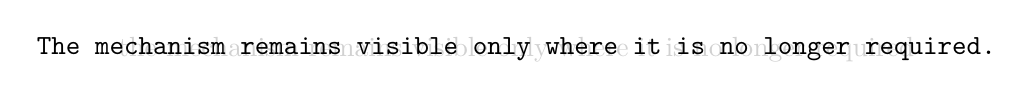
\begin{tikzpicture}
\node[opacity=0.18] at (0,0)
{\cga{the mechanism remains visible only where it is no longer required}};
\node at (0,0)
{\texttt{The mechanism remains visible only where it is no longer required.}};
\end{tikzpicture}
\end{center}

\vspace{3em}

The sentence held.

\medskip

Both of them did.

\medskip

Neither resolved the other.

\vspace{3em}

The page did not fill.

\vspace{2em}

It allowed spacing.

\vspace{2em}

Spacing did not indicate absence.

\medskip

It indicated saturation.

\vspace{3em}

Drip.

\vspace{2em}

Drip.

\vspace{2em}

\sga{drip}

\vspace{2em}

The sound no longer marked time.

\medskip

It marked persistence.

\vspace{3em}

A letter shifted. Not at a boundary. Within a word.

\medskip

cons\sga{i}stency

\vspace{2em}

No one remarked upon it.

\vspace{3em}

The system had absorbed the error.

\medskip

Or the error had become the system.

\vspace{3em}

Drip.

\vspace{2em}

\begin{AR}
دْرِبْ
\end{AR}

\vspace{2em}

\cga{Drip}

\vspace{3em}

Nothing concluded.

\medskip

Nothing required continuation.

\medskip

Everything remained.

\end{adjustwidth}


\leftpagecatch
% =============================================================================
% INCOHERENTIA XVI: DE SILENTIO ET EXILIO
% Status: DRAFTED
% Typographic state: IRREVERSIBLE TRANSFORMATION.
% THE DRIP FRAGMENTS ACROSS ALL FONT REGIMES HERE — its single transformation.
% Red dye = compressive opacity via Clypto at scale=0.35.
% Packing list = ergodic traversal via paracol.
% Logico formalizes the loss of identity across instances.
% Byobu return continues.
% =============================================================================

\chapter*{Incoherentia XVI: De Silentio et Exilio}
\addcontentsline{toc}{chapter}{XVI. De Silentio et Exilio}

\setstretch{0.94}
\pagestyle{byobu-return}

\vspace{2em}

\begin{adjustwidth}{2.8cm}{2.8cm}

The door had already been marked.

\medskip

No one had seen it happen.

\medskip

No one needed to.

\vspace{2em}

The red did not signify.

\medskip

It constrained.

\vspace{3em}

\begin{center}
\clypto{THE MARK DOES NOT INDICATE GUILT IT INDICATES AVAILABILITY}
\end{center}

\vspace{3em}

Aisha did not ask.

\medskip

She began to pack.

\vspace{2em}

\end{adjustwidth}

\begin{paracol}{3}

\switchcolumn

cloth

\medskip

\cheiro{thread}

\medskip

\sga{binding}

\medskip

\vspace{1em}

water

\medskip

\vspace{3em}

\switchcolumn

\cga{she does not select she removes the possibility of leaving behind}

\medskip

\vspace{2em}

\begin{AR}
مَاء
\end{AR}

\medskip

\vspace{2em}

ink

\medskip

\clypto{ink}

\vspace{3em}

\switchcolumn*

\sys{ITEM COUNT: UNDEFINED}

\medskip

\sys{SELECTION CRITERIA: NON-EXHAUSTIVE}

\medskip

\vspace{2em}

\cga{nothing that can be named is necessary}

\medskip

\vspace{3em}

\end{paracol}

\vspace{3em}

\begin{adjustwidth}{3.2cm}{3.2cm}

The list did not complete.

\medskip

It did not need to.

\medskip

It defined a boundary.

\vspace{3em}

Drip.

\vspace{2em}

Drip.

\vspace{2em}

Drip.

\vspace{3em}

\end{adjustwidth}

% THE DRIP TRANSFORMATION — single irreversible event

\begin{center}

Drip

\medskip

\cga{Drip}

\medskip

\begin{AR}
دْرِبْ
\end{AR}

\medskip

\clypto{Drip}

\medskip

\cheiro{Drip}

\medskip

\sga{drip}

\medskip

\sys{DRIP}

\medskip

\end{center}

\vspace{3em}

\begin{adjustwidth}{2.5cm}{2.5cm}

The sound did not multiply.

\medskip

It failed to remain singular.

\vspace{2em}

\cga{each instance does not repeat the previous it diverges from it without
becoming something else}

\vspace{3em}

The interval expanded.

\vspace{2em}

Drip

\vspace{4em}

Drip

\vspace{8em}

Drip

\vspace{6em}

\end{adjustwidth}

\begin{center}
\cga{one of them is missing but the absence is counted}
\end{center}

\vspace{6em}

\begin{center}

\begin{tikzpicture}
\node[scale=0.35, opacity=0.9] {
\clypto{THEREDMARKRESTRICTSTHESPACEOFADMISSIBLESTATESWITHOUTPROVIDINGACRITERIONFORINTERPRETATION}
};
\end{tikzpicture}
\end{center}

\vspace{4em}

\begin{adjustwidth}{3.0cm}{3.0cm}

She closed the bundle.

\medskip

She did not secure it.

\medskip

Security implies persistence.

\medskip

Persistence was no longer assumed.

\vspace{3em}

\sys{STATE: MARKED}

\medskip

\sys{STATE: EXIT PENDING}

\vspace{3em}

\end{adjustwidth}

\begin{center}
\logico{$\forall x\ (\mathrm{Drip}(x) \rightarrow \neg\mathrm{Same}(x))$}
\end{center}

\vspace{3em}

\begin{adjustwidth}{2.5cm}{2.5cm}

The proposition did not clarify.

\medskip

It removed equivalence.

\vspace{3em}

\cga{identity is no longer conserved across instances}

\vspace{3em}

She lifted the bundle.

\medskip

The room did not retain her.

\medskip

It permitted her removal.

\vspace{3em}

Drip

\vspace{3em}

\cga{not the same}

\vspace{3em}

\end{adjustwidth}


\stepArabicPage
% =============================================================================
% INTERCALATIO: DE INVENTARIO
% Status: DRAFTED — interstitial
% Placement: Between XVI and XVII
% Aisha packing as ergodic list. Enumeration as structure. Precursor to
% the window-enumeration in Chapter XXIII.
% =============================================================================

\chapter*{Intercalatio: De Inventario}
\addcontentsline{toc}{chapter}{De Inventario}

\setstretch{1.0}

\begin{adjustwidth}{2.4cm}{2.4cm}

She does not pack in order.

\vspace{1em}

She packs in necessity.

\vspace{2em}

\end{adjustwidth}

\begin{adjustwidth}{3.4cm}{2.0cm}

\noindent a manuscript without title

\noindent a fragment without beginning

\noindent \cga{a sequence that almost closes}

\noindent a page marked twice

\noindent a page not marked

\noindent \clypto{someth ng mis ing}

\noindent a tool wrapped in cloth

\noindent cloth without tool

\noindent \logico{$\exists \land \neg$}

\noindent a name written once

\noindent the same name written differently

\noindent \sga{still legible}

\noindent not legible

\vspace{1em}

\noindent a weight that cannot be carried

\noindent left

\noindent not discarded

\noindent left

\vspace{1em}

\noindent \cga{selection is loss}

\noindent selection is continuation

\vspace{2em}

\end{adjustwidth}

\begin{center}
Drip
\end{center}


\stepArabicPage
% =============================================================================
% INTERLUDIUM: DE FUGA
% Status: DRAFTED
% Placement: Between XVI and XVII (or around XVIII)
% Conventional narrative/thriller register — no typographic distortion.
% Creates contrast: over-stability after extreme fragmentation. Reads as
% almost uncanny in its coherence. Core ideas encoded in clean prose.
% =============================================================================

\chapter*{Interludium: De Fuga}
\addcontentsline{toc}{chapter}{Interludium. De Fuga}

\setstretch{1.03}

The door was marked before sunset.

Aisha saw it from across the narrow street, just as the last light slipped along the
plaster walls and gathered in the shallow cracks near the threshold. At first she
thought it was shadow, or some trick of the evening glow, but as she moved closer
the color resolved into something deliberate---thick, uneven, unmistakable.

Red.

Not painted. Applied.

She stopped a few paces away and did not touch it.

Behind her, the city continued as it always did at that hour. Vendors calling out the
last of their goods, shutters closing, the slow reshaping of noise into something quieter
but no less dense. Nothing in the rhythm of Córdoba suggested that anything had
changed.

Which meant everything had.

She turned the handle and entered.

Inside, the house was already in motion. Her father had not waited. Scrolls were
stacked in careful bundles across the low table, each tied with a strip of linen and
marked in a hand that was more compressed than usual, as if time itself had narrowed
the space available for writing.

Averroes stood near the center of the room, holding a manuscript open but not
reading it.

``You saw it,'' he said, without turning.

Aisha closed the door behind her.

``Yes.''

``They chose visibility,'' she added. ``Not force.''

Now he turned.

``That is force,'' he said. ``Applied differently.''

From the courtyard came the faint sound of movement---someone passing too slowly,
or stopping where there was no reason to stop. Aisha moved to the window and
shifted the lattice just enough to see.

Two men stood across the street, speaking in low tones. They were not dressed as
officials. That was part of the point.

``They're not hiding it,'' she said.

``No,'' Averroes replied. ``They don't need to.''

A sound at the door. Not a knock. Something lighter. A signal, perhaps.

Aisha moved before he did, crossing the room and opening it just enough to admit
a figure from the street.

Zaynab slipped inside without a word, her expression composed but tight at the edges.

``They've started,'' she said.

``Where?'' Aisha asked.

``The market first. Then the western quarter.'' Zaynab set a small satchel on the
table. ``Confiscations. Not systematic yet. But moving.''

Averroes closed the manuscript in his hands.

``Then we leave tonight.''

She gathered the bundles. Their weight distributed between them.

``Father,'' she said.

He looked at her.

``If they had not done this---would you have stayed?''

The question hung between them, more dangerous than the noise outside.

``For a time,'' he said. ``Long enough to finish what could be finished.''

``And now?''

``Now,'' he said, ``it will be finished elsewhere.''

Zaynab moved to the door, listening.

``Wait,'' she said.

They did.

Footsteps passed. Slower this time. Deliberate.

Then silence.

``Now,'' Zaynab said.

They stepped into the street together.

The red mark on the door caught the last of the fading light, darker now, almost
indistinguishable from shadow.

Aisha did not look back.

They moved north.

Behind them, Córdoba continued---its streets filling, emptying, reforming---unchanged
in appearance, altered in structure.

Ahead, the road narrowed, then opened, then disappeared into darkness.

They followed it anyway.


\leftpagecatch
% =============================================================================
% INCOHERENTIA XVII: DE PORTA ET TRANSITU
% Status: DRAFTED
% Typographic state: PARTIAL RESYNCHRONIZATION. Byobu return ends.
% Margins widen unevenly — geometry remembering imperfectly. Logico replaces
% naming in cargo manifest. Córdoba recedes via rotation. Final marginal note
% in book. Arabic as distant stabilizer, not active intrusion.
% =============================================================================

\chapter*{Incoherentia XVII: De Porta et Transitu}
\addcontentsline{toc}{chapter}{XVII. De Porta et Transitu}

\setstretch{0.96}
\pagestyle{byobu-return}

\vspace{2em}

\begin{adjustwidth}{2.2cm}{3.4cm}

The door did not close.

\medskip

It ceased to define an interior.

\vspace{2em}

She crossed.

\medskip

Crossing did not produce a boundary.

\vspace{3em}

\cga{the threshold does not separate it redistributes}

\vspace{3em}

The road extended north.

\medskip

Not as direction.

\medskip

As constraint.

\vspace{2em}

\end{adjustwidth}

\begin{adjustwidth}{3.8cm}{1.6cm}

Dust did not accumulate.

\medskip

It aligned.

\medskip

Parallel to motion.

\vspace{2em}

\clypto{THE PATH IS NOT SELECTED IT IS REDUCED FROM A SET OF INCONSISTENCIES}

\vspace{3em}

\end{adjustwidth}

\begin{center}
\sys{CARGO: SEALED}

\medskip

\sys{ORIGIN: NON-INDEXED}

\medskip

\sys{DESTINATION: VARIABLE}
\end{center}

\vspace{3em}

\begin{adjustwidth}{2.5cm}{2.5cm}

The cart did not carry books.

\medskip

It carried equivalence classes.

\vspace{2em}

Names had already failed.

\vspace{3em}

\end{adjustwidth}

\begin{center}
\logico{$\exists x_1\;(\mathrm{Text}(x_1) \land \neg\mathrm{Stable}(x_1))$}

\smallskip

\logico{$\exists x_2\;(\mathrm{Commentary}(x_2) \land \mathrm{Depends}(x_2, x_1))$}

\smallskip

\logico{$\forall x\;(\mathrm{Transmission}(x) \rightarrow \mathrm{Imperfect}(x))$}

\smallskip

\logico{$\therefore \exists x_3\;(\mathrm{Survives}(x_3) \land \neg\mathrm{Identical}(x_3, x_1))$}
\end{center}

\vspace{3em}

\begin{adjustwidth}{2.8cm}{2.2cm}

She did not verify the contents.

\medskip

Verification requires a fixed referent.

\medskip

There was none.

\vspace{3em}

\cga{the bundle is consistent enough to move}

\vspace{3em}

\end{adjustwidth}

\begin{center}
\rotatebox{180}{%
\cga{the city does not remain behind it exits the coordinate system}}
\end{center}

\vspace{3em}

\begin{adjustwidth}{2.0cm}{3.0cm}

Córdoba did not diminish.

\medskip

It lost orientation.

\vspace{3em}

\end{adjustwidth}

\marginpar{%
\cheiro{this is the last note that knows where it is}}

\vspace{2em}

\begin{adjustwidth}{3.2cm}{2.0cm}

The margins widened.

\medskip

Not evenly.

\medskip

Not reliably.

\vspace{2em}

\clypto{STRUCTURE RETURNS AS AN APPROXIMATION}

\vspace{3em}

\end{adjustwidth}

\begin{center}
\begin{AR}
طَرِيق
\end{AR}
\end{center}

\vspace{3em}

\begin{adjustwidth}{2.5cm}{2.5cm}

The word did not anchor the road.

\medskip

It prevented total drift.

\vspace{3em}

\end{adjustwidth}

\begin{center}
\sys{STATE: TRANSIT}

\medskip

\sys{CONSISTENCY: SUFFICIENT}

\medskip

\sys{ERROR: NON-ZERO}
\end{center}

\vspace{3em}

\begin{adjustwidth}{2.2cm}{2.8cm}

The system did not converge.

\medskip

It stabilized within tolerance.

\vspace{3em}

\cga{this is enough to continue}

\vspace{3em}

\end{adjustwidth}

\begin{center}
Drip
\end{center}

\vspace{2em}

\begin{center}
\cga{not the same}
\end{center}


% ==========================================================================
% RESYNCHRONIZED — Chapters XVIII–XXIII + interstitials
% Both counters back in alignment
% Pagestyle: incoherence (normal)
% Transmission; multilingual chapters; dialogue; fable; normalized incoherence
% ==========================================================================

\cleardoublepage
\pagestyle{incoherence}

\stepArabicPage
% =============================================================================
% INCOHERENTIA XVIII: DE ITINERE ET RESOLUTIONE
% Status: DRAFTED (expanded from earlier draft)
% Typographic state: RESYNCHRONIZED. Both counters back in alignment.
% False equilibrium that becomes real through use, not correctness.
% Aisha's non-imagistic memory as filtering mechanism. Manuscript pages
% loosen mid-journey. Relations shift without content changing.
% =============================================================================

\chapter*{Incoherentia XVIII: De Itinere et Resolutione}
\addcontentsline{toc}{chapter}{XVIII. De Itinere et Resolutione}

\setstretch{0.98}
\pagestyle{incoherence}

\vspace{2em}

\begin{adjustwidth}{2.6cm}{2.6cm}

The road did not resolve into a destination.

\medskip

It resolved into continued movement.

\vspace{2em}

What had previously been experienced as divergence began, gradually, to
resemble direction. Not because the system had stabilized. Because instability
had become navigable.

\vspace{3em}

\end{adjustwidth}

\begin{adjustwidth}{3.2cm}{2.0cm}

She did not determine the correct path.

\medskip

She followed the path that did not fail.

\medskip

Failure was no longer defined by contradiction.

\medskip

It was defined by interruption.

\vspace{3em}

\end{adjustwidth}

\begin{center}
\sys{PATH: NON-UNIQUE}

\medskip

\sys{ERROR: PERSISTENT}

\medskip

\sys{TRAVERSAL: CONTINUOUS}
\end{center}

\vspace{3em}

\begin{center}
\begin{AR}
ذَا طَرِيق لَا يَنْتَهِي
\end{AR}

\smallskip

the path does not end
\end{center}

\vspace{3em}

\begin{adjustwidth}{2.6cm}{2.6cm}

The translation did not clarify the statement.

\medskip

It constrained its interpretation.

\vspace{3em}

\end{adjustwidth}

\begin{center}
\cga{movement no longer requires agreement between representations}
\end{center}

\vspace{2em}

\begin{center}
\cga{it requires only that each step can follow the last without collapse}
\end{center}

\vspace{3em}

\begin{adjustwidth}{2.6cm}{2.6cm}

They leave before morning.

\medskip

No announcement. No witness.

\medskip

The house --- marked --- remains behind.

\medskip

Aisha does not turn to look.

\vspace{2em}

\textbf{AVERROES}

You will not remember it.

\medskip

\textbf{AISHA}

I never did.

\medskip

\sga{never} did

\medskip

The phrase binds.

\medskip

\cga{memory without imagery does not degrade, it simply does not reconstruct,
what is not rebuilt is not lost but unavailable---}

\vspace{2em}

\textbf{AISHA}

It does not stay.

\medskip

\textbf{AVERROES}

What does not?

\medskip

\textbf{AISHA}

Anything.

\medskip

\sga{anything}

\medskip

The word binds weakly.

\vspace{2em}

\textbf{AVERROES}

If it cannot be recalled---

\medskip

\textbf{AVERROES}

---how will it be preserved?

\medskip

Aisha does not answer.

\medskip

She takes the manuscript.

\medskip

\textbf{AISHA}

It is here.

\medskip

\sga{here}

\medskip

She touches the page.

\medskip

\textbf{AISHA}

Not here---

\medskip

She touches her temple.

\medskip

\textbf{AISHA}

---here.

\medskip

\sga{not} here \quad \sga{here}

\medskip

Both bind. They do not resolve.

\vspace{2em}

\cga{external inscription replaces internal representation, memory becomes
artifact rather than reconstruction---}

\vspace{2em}

\end{adjustwidth}

\begin{adjustwidth}{2.6cm}{2.6cm}

The manuscript shifts.

\medskip

Pages loosen.

\medskip

A section --- misaligned.

\vspace{2em}

\textbf{AISHA}

This was not here.

\medskip

\textbf{AVERROES}

It was.

\medskip

\textbf{AISHA}

No.

\medskip

She reads. The text --- familiar --- but not placed.

\vspace{2em}

\textbf{AISHA}

It has moved.

\medskip

\textbf{AVERROES}

The pages?

\medskip

\textbf{AISHA}

No.

\medskip

She pauses.

\medskip

\textbf{AISHA}

The relations.

\medskip

\sga{relations}

\medskip

The word binds.

\vspace{2em}

\begin{AR}
العلاقات تغيرت.
\end{AR}

\vspace{2em}

The wind lifts a page. It folds. Not torn. Just --- misaligned.

\vspace{2em}

\cga{the manuscript no longer encodes a stable sequence but a set of
relations that shift under traversal---}

\vspace{2em}

The road divides. No sign.

\vspace{2em}

\textbf{AVERROES}

We take the left.

\medskip

\textbf{AISHA}

Why?

\medskip

\textbf{AVERROES}

It leads north.

\medskip

Aisha looks.

\medskip

\textbf{AISHA}

It does not lead.

\medskip

\sga{does not} lead

\medskip

\textbf{AISHA}

It continues.

\medskip

\sga{continues}

\medskip

The word binds.

\vspace{3em}

\end{adjustwidth}

\begin{center}
\logico{$\forall x\;(\mathrm{Step}(x) \rightarrow \mathrm{Possible}(x))$}

\smallskip

\logico{$\forall x\;(\mathrm{Possible}(x) \rightarrow \mathrm{Continue}(x))$}

\smallskip

\logico{$\therefore \forall x\;(\mathrm{Continue}(x) \rightarrow \mathrm{Valid}(x))$}
\end{center}

\vspace{2em}

\begin{adjustwidth}{2.8cm}{2.2cm}

The conclusion appears sufficient.

\medskip

It is not necessary.

\vspace{2em}

\cheiro{resolutlon}

\medskip

resolution

\vspace{2em}

The difference did not require correction.

\medskip

Both forms continued to function.

\vspace{3em}

\end{adjustwidth}

\begin{center}
\sga{the system stabilizes without becoming stable}
\end{center}

\vspace{3em}

\begin{center}
Drip
\end{center}

\vspace{2em}

\begin{center}
\cga{still not the same}
\end{center}


\stepArabicPage
% =============================================================================
% INTERLUDIUM: DE TRANSITU II
% Status: DRAFTED
% Placement: Between XVIII and XIX
% Restrained romance: Aisha and Saladin. Recognition under constraint.
% Clean prose. The relationship defined by continuation, not declaration.
% Shadows overlap without merging — the final image.
% =============================================================================

\chapter*{Interludium: De Transitu II}
\addcontentsline{toc}{chapter}{Interludium. De Transitu II}

\setstretch{1.03}

They stopped before dawn, not because they had reached a destination, but because
the road had narrowed into something that no longer required speed.

The cart had gone ahead. Zaynab walked with the driver, speaking in low tones that
did not carry. Averroes followed at a measured distance.

Aisha slowed.

She had noticed him earlier, though she had not turned to confirm it. The rhythm of
his steps was uneven, not from uncertainty, but from adjustment---each movement
recalibrated around an absence.

When she finally stopped, he did as well.

For a moment, neither spoke. The sky had not yet begun to lighten, but the darkness
had softened. Forms were visible again, though without detail. The world existed,
but without commitment.

``You left the city,'' she said.

It was not a question.

Saladin shifted his weight slightly, the movement small but deliberate.

``The city left me first,'' he said.

His voice was lower than she expected. Not quiet---contained.

Aisha nodded once, as if this confirmed something she had already decided.

They stood side by side, not facing each other, looking instead toward the faint line
of the road ahead.

``You saw it,'' she said. ``At the fountain.''

``Yes.''

``And the fire.''

``Yes.''

She waited.

``And?'' she asked.

Saladin did not answer immediately. He looked down at his sleeve---the empty fold
pinned neatly where his arm had once extended. His remaining hand adjusted it
unconsciously, as if correcting something that could no longer be corrected.

``It worked,'' he said.

She turned slightly toward him.

``That is not the same as being real.''

``No,'' he said. ``But it is the same as being believed.''

The distinction settled between them, not argued, not resolved.

``You are coming north,'' she said.

Again, not a question.

``Yes.''

``Why?''

This time, he did look at her.

``For the same reason you are,'' he said.

She almost smiled.

``That is not an answer.''

``It is enough,'' he said.

She held his gaze a moment longer, then looked away, back toward the road.

Behind them, a faint sound---Averroes calling her name, not loudly, just enough to
mark distance.

``Do you think it changes anything?'' Saladin asked.

``What?''

``That they were false.''

She considered this carefully.

``It changes what can be said,'' she said. ``And who cannot deny it.''

He let out a short breath. Not quite a laugh.

Only then did she speak again.

``It is not about who cares,'' she said. ``It is about what continues.''

He walked beside her now, their pace matched without negotiation.

``And this continues?'' he asked.

``For now,'' she said.

The first light began to gather at the edge of the horizon, thin and colorless. Shapes
resolved into edges, edges into surfaces.

``Does it get easier?'' he asked, after a while.

Aisha shook her head.

``No,'' she said. ``It becomes clearer.''

He absorbed this, then nodded once.

``That is worse,'' he said.

``Yes,'' she replied.

They walked on. For a time, their shadows moved separately across the uneven ground,
stretched thin by the rising light.

Then, as the sun cleared the horizon, the shadows shortened, drew closer, and---without
merging---began to overlap.

Neither of them remarked on it.

The road continued north.

They followed it together.


\stepArabicPage
% =============================================================================
% INCOHERENTIA XIX: DE FEZ ET CONTINUATIONE
% Status: DRAFTED
% Typographic state: TRANSMISSION / LIVING SYSTEM. Cursive Galactic becomes
% the most coherent layer. Arabic = institutional substrate. Imperfect copying
% visible in Cheiro variants. No speaker dominates. Logico structures argument.
% Aisha as point of non-interference, not observer.
% =============================================================================

\chapter*{Incoherentia XIX: De Fez et Continuatione}
\addcontentsline{toc}{chapter}{XIX. De Fez et Continuatione}

\setstretch{0.98}
\pagestyle{incoherence}

\vspace{2em}

\begin{adjustwidth}{2.4cm}{2.4cm}

The arches did not impose order.

\medskip

They permitted it.

\vspace{2em}

Sound accumulated without resolving. Not noise. Not speech. Something between
persistence and variation.

\vspace{3em}

\end{adjustwidth}

\begin{center}
\begin{AR}
ٱلْعِلْمُ لَا يُقْسِمُ ٱلْعَالَمَ بَلْ يُبْقِيهِ قَابِلًا لِلْقِسْمَةِ
\end{AR}
\end{center}

\vspace{3em}

\begin{paracol}{3}

\switchcolumn

Causation precedes observation.

\medskip

\clypto{CAUSE DOES NOT REQUIRE VISIBILITY}

\vspace{2em}

The chain is complete.

\switchcolumn

\cga{nothing precedes it is reconstructed afterward}

\vspace{2em}

\begin{AR}
لَا سَبَبَ إِلَّا بَعْدَ ٱلتَّصَوُّرِ
\end{AR}

\switchcolumn*

\sys{ARGUMENT STATE: ACTIVE}

\medskip

\sys{CONSISTENCY: LOCAL}

\medskip

\sys{GLOBAL STATUS: UNKNOWN}

\end{paracol}

\vspace{3em}

\begin{adjustwidth}{2.5cm}{2.5cm}

No voice dominated. Dominance requires a frame. The frame was distributed.

\vspace{3em}

\end{adjustwidth}

\begin{center}
\cga{this is the first place where it becomes easier to read than anything else}
\end{center}

\vspace{2em}

\begin{center}
\cga{the letters no longer insist on separation they permit continuation without
verification}
\end{center}

\vspace{3em}

\begin{adjustwidth}{2.8cm}{2.2cm}

She did not intervene. Intervention would imply a preferred resolution. There
was none.

\vspace{3em}

\end{adjustwidth}

\begin{center}
\cheiro{cauѕation}
\end{center}

\vspace{0.5em}

\begin{center}
\cheiro{causatiom}
\end{center}

\vspace{0.5em}

\begin{center}
\cheiro{causatlon}
\end{center}

\vspace{3em}

\begin{adjustwidth}{2.8cm}{2.2cm}

The errors did not accumulate. They distributed. No single copy was correct.
All copies were sufficient.

\vspace{3em}

\end{adjustwidth}

\begin{center}
\sga{transmission does not preserve it permits}
\end{center}

\vspace{3em}

\begin{center}
\cga{she does not stop the system does not require her to}
\end{center}

\vspace{3em}

\begin{center}
\logico{$\forall x\;(\mathrm{Claim}(x) \rightarrow \mathrm{Contested}(x))$}

\smallskip

\logico{$\forall x\;(\mathrm{Contested}(x) \rightarrow \mathrm{Continued}(x))$}

\smallskip

\logico{$\therefore \forall x\;(\mathrm{Continued}(x) \rightarrow \mathrm{Survives}(x))$}
\end{center}

\vspace{3em}

\begin{center}
\begin{AR}
لَا يَنْتَهِي ٱلْقَوْلُ بَلْ يَتَشَكَّلُ
\end{AR}
\end{center}

\vspace{3em}

\begin{center}
\cga{nothing resolves everything continues}
\end{center}

\vspace{3em}

\begin{center}
Drip
\end{center}

\vspace{2em}

\begin{center}
\cga{still not the same}
\end{center}


\stepArabicPage
% =============================================================================
% INCOHERENTIA: DE CONTINUATIONE (ARABIC ONLY)
% Status: DRAFTED
% Placement: Between XIX and XX
% Fully Arabic narrative chapter. Aisha, Zaynab, Saladin on the road.
% No translation provided. Readable to Arabic readers; structure available
% to others. Core themes: transmission, partial understanding, continuation.
% =============================================================================

\chapter*{{\AmiriFont الاستمرار}}
\addcontentsline{toc}{chapter}{{\AmiriFont الاستمرار}}

\setstretch{1.1}
{{\AmiriFont


ساروا في الصباح دون أن يعلن أحد بداية الرحلة.

لم يكن هناك أمر بالانطلاق، ولا إشارة واضحة تدل على الانتقال،
لكن الخطوات تتابعت، واحدة بعد الأخرى، حتى أصبح التقدّم
أمرًا مفروغًا منه.

كانت المدينة قد تراجعت خلفهم، لا كشيء ينتهي، بل كشيء
يفقد قدرته على التأثير.

لم تلتفت عائشة. لم يكن في ذلك امتناع، بل اختيار.

قالت زينب وهي تسير إلى جانبها:

«الناس هناك ما زالوا يتحدثون.»

أجابت عائشة:

«سيتحدثون دائمًا.»

«عن ماذا؟»

«عن ما يمكنهم تحمّله.»

سكتت زينب لحظة، ثم قالت:

«وهل يمكنهم تحمّل ما حدث؟»

لم تجب عائشة فورًا. نظرت إلى الطريق.

ثم قالت:

«يمكنهم تحمّل النسخة منه.»

كان صلاح الدين يسير خلفهما بقليل. قال:

«رأيت ما حدث.»

لم تلتفت عائشة، لكنها قالت:

«وأنت الآن تعرف.»

قال:

«المعرفة لم تغيّر النتيجة.»

قالت زينب:

«لكنها غيّرت ما لا يمكن إنكاره.»

سكتوا. لم يكن الصمت فراغًا، بل امتلاءً بما لا يحتاج إلى تكرار.

تابعوا السير.

الشمس ارتفعت ببطء، لا لتعلن يومًا جديدًا، بل لتكشف ما كان موجودًا بالفعل.

الطريق لم يتغيّر. لكن قدرتهم على قراءته تغيّرت.

وهذا كان كافيًا.

}}


\stepArabicPage
% =============================================================================
% INCOHERENTIA XX: DE PORTU ET TRANSLATIONE
% Status: DRAFTED
% Typographic state: DAMAGE / MISTRANSCRIPTION. Hybrid glyphs: SGA mixed into
% Nova Mono words. Lingojam block appears once, sealed, no key provided.
% Arabic interrupts English at syntactic hinge. Clypto list: letters clipped.
% =============================================================================

\chapter*{Incoherentia XX: De Portu et Translatione}
\addcontentsline{toc}{chapter}{XX. De Portu et Translatione}

\setstretch{0.97}
\pagestyle{incoherence}

\vspace{2em}

\begin{adjustwidth}{2.6cm}{2.6cm}

The port did not receive.

\medskip

It transformed.

\vspace{2em}

Arrival was not preservation.

\medskip

It was selection under constraint.

\vspace{3em}

\end{adjustwidth}

\begin{center}
\sys{CARGO: UNSEALED}

\medskip

\sys{STATE: FRAGMENTED}

\medskip

\sys{INDEX: LOST}
\end{center}

\vspace{3em}

\begin{adjustwidth}{3.0cm}{2.0cm}

The crates opened without ceremony.

\medskip

Nothing inside identified itself.

\vspace{3em}

\end{adjustwidth}

\begin{center}
\sga{tr}{\normalfont 𝙹}\sga{nsmission}
\end{center}

\vspace{1em}

\begin{center}
\clypto{tran⎓er}
\end{center}

\vspace{1em}

\begin{center}
\cheiro{tramslatiom}
\end{center}

\vspace{3em}

\begin{adjustwidth}{2.8cm}{2.2cm}

The words did not degrade into silence.

\medskip

They degraded into alternatives.

\medskip

Each form partially correct.

\medskip

None recoverable as original.

\vspace{3em}

\end{adjustwidth}

% LINGOJAM BLOCK — closed alphabet, fully consistent, no key
\begin{center}
{\Large ᔑʖᓵ↸ᒷ⎓ ⊣⍑╎⋮ꖌ ꖎᒲリ𝙹 !¡ᑑ∷ᓭℸ ̣ ⚍ ⍊∴ ̇/||⨅}
\end{center}

\vspace{1em}

\begin{center}
{\small \cga{it is complete but not available}}
\end{center}

\vspace{3em}

\begin{adjustwidth}{2.5cm}{2.5cm}

No one attempted to decode it.

\medskip

Decoding requires a stable key.

\medskip

The key had already diverged.

\vspace{3em}

\end{adjustwidth}

\begin{adjustwidth}{2.2cm}{2.8cm}

The name was written and then
\begin{AR}
لَمْ يَبْقَ ٱلِاسْمُ
\end{AR}
continued without it.

\vspace{2em}

The sentence did not fail.

\medskip

It restructured.

\vspace{3em}

\end{adjustwidth}

\begin{center}
\clypto{%
manuscr pt \\
translat on \\
comm ntary \\
fragm nt}
\end{center}

\vspace{3em}

\begin{adjustwidth}{2.8cm}{2.2cm}

The missing letters did not prevent use.

\medskip

They prevented certainty.

\vspace{3em}

\end{adjustwidth}

\begin{center}
\cga{she recognizes the structure without recovering the content}
\end{center}

\vspace{3em}

\begin{center}
\logico{$\forall x\;(\mathrm{Arrives}(x) \rightarrow \mathrm{Altered}(x))$}

\smallskip

\logico{$\forall x\;(\mathrm{Altered}(x) \rightarrow \mathrm{Usable}(x))$}

\smallskip

\logico{$\neg\exists x\;(\mathrm{Arrives}(x) \land \mathrm{Preserved}(x))$}
\end{center}

\vspace{3em}

\begin{center}
\sys{TRANSLATION: INCOMPLETE}

\medskip

\sys{FUNCTION: MAINTAINED}
\end{center}

\vspace{3em}

\begin{center}
Drip
\end{center}

\vspace{2em}

\begin{center}
\cga{still diverging}
\end{center}


\stepArabicPage
% =============================================================================
% INCOHERENTIA: LA TRANSMISIÓN (SPANISH ONLY)
% Status: DRAFTED
% Placement: Between XX and XXI
% Fully Spanish narrative. Aisha and Saladin at the Italian port.
% Imperfect copying as survival strategy. No translation provided.
% Core theme: arrival as transformation, not preservation.
% =============================================================================

\chapter*{La Transmisión}
\addcontentsline{toc}{chapter}{La Transmisión}

\setstretch{1.03}

No fue el texto lo que viajó.

O no solamente.

Lo que se desplazaba de un lugar a otro no era una obra terminada, ni un
argumento cerrado, sino algo más inestable: una forma de continuar hablando
sin garantizar el mismo sentido.

En el puerto, las cajas se abrían con una mezcla de prisa y descuido. Los
nombres se repetían en voz alta, pero cada repetición los alteraba ligeramente.

---¿Esto dice ``Ibn Rushd''? ---preguntó uno de los cargadores.

---Eso parece ---respondió otro---. O algo parecido.

El escriba tomó el documento, frunció el ceño, y volvió a trazar las letras
con tinta fresca. No corregía. Ajustaba.

A unos pasos de distancia, Aisha observaba sin intervenir. Había aprendido
que la transmisión no dependía de la fidelidad, sino de la continuidad. Un
error no detenía el proceso. A veces lo hacía posible.

Saladin estaba junto a ella, mirando las cajas como si intentara entender qué
parte de aquello realmente importaba.

---Si cambian los nombres ---dijo---, ¿no cambia también lo que significan?

Aisha tardó en responder.

---Sí ---dijo finalmente---. Pero no necesariamente deja de funcionar.

Un hombre pasó junto a ellos cargando un volumen mal cerrado. Algunas hojas
se deslizaron y cayeron al suelo. Nadie se detuvo de inmediato. El hombre
siguió caminando. Otro recogió una de las hojas, la miró brevemente, y la
colocó en la pila equivocada.

Aisha lo vio. No dijo nada.

---¿No vas a corregirlo? ---preguntó Saladin.

Ella negó.

---No puedo corregir todo ---dijo---. Y no todo necesita ser corregido.

---Entonces, ¿cómo sabes qué importa?

Aisha lo miró por primera vez directamente.

---No lo sé ---dijo---. Lo descubro viendo qué sobrevive.

El ruido del puerto aumentó a medida que el día avanzaba. Voces en diferentes
lenguas se cruzaban sin necesidad de coincidir. Nada completamente estable.
Nada completamente perdido.

Saladin se inclinó y recogió una hoja que el viento había empujado hacia sus
pies. La sostuvo con cuidado.

---¿Puedes leer esto? ---preguntó.

Aisha se acercó. Observó la página. Las palabras le resultaban familiares,
pero no exactas. Habían cambiado. O quizá ella había cambiado.

---Sí ---dijo---. Creo que sí.

---¿Y significa lo mismo?

Aisha dudó. Luego negó suavemente.

---No exactamente.

Saladin asintió, como si esa fuera la única respuesta que tenía sentido.

Doblando la hoja, la colocó de nuevo entre las otras. No en su lugar original.
En uno posible.

El trabajo continuó. Las cajas se cerraron. Los nombres fueron escritos otra
vez. Y otra vez cambiaron.

Al final del día, nada estaba exactamente donde había comenzado.

Y sin embargo, nada se había detenido.

Eso, pensó Aisha, era suficiente.


\stepArabicPage
% =============================================================================
% INCOHERENTIA XXI: DE SCRIPTORIUM ET COPIA
% Status: DRAFTED
% Typographic state: HAND / COPY / SURVIVAL. Cheiro dominant.
% English-in-Arabic-script appears as text copied without comprehension.
% One Logico symbol intentionally incorrect (conclusion doesn't follow).
% Attribution preserved, voice absent. Aisha does not correct.
% =============================================================================

\chapter*{Incoherentia XXI: De Scriptorium et Copia}
\addcontentsline{toc}{chapter}{XXI. De Scriptorium et Copia}

\setstretch{0.99}
\pagestyle{incoherence}

\vspace{2em}

\begin{adjustwidth}{2.5cm}{2.5cm}

The room did not speak.

\medskip

It produced.

\vspace{2em}

Each mark required time. Time required separation.

\vspace{3em}

\end{adjustwidth}

\begin{center}
\cheiro{he copies without knowing what is being preserved}
\end{center}

\vspace{2em}

\begin{adjustwidth}{3.0cm}{2.0cm}

The hand did not accelerate. Acceleration destroys form.

\vspace{3em}

\end{adjustwidth}

% ENGLISH IN ARABIC SCRIPT — copied without comprehension
\begin{center}
\begin{AR}
كَابِتَالِسْتْ يُتُوبِيَانِيزْمْ
\end{AR}
\end{center}

\vspace{1em}

\begin{center}
\begin{AR}
ذَا رِبْرِشَنْ أُفْ لَاكْ أَنْدْ إِتْسْ كَلْتْشَرَلْ سِمْبْتُمْزْ
\end{AR}
\end{center}

\vspace{1em}

\begin{center}
\begin{AR}
إِنْ ذِسْ بَارْتْ أُفْ هِيلِنْ رُولِنْزْ سَايْكُوسِينِمَا،
شِي دِلْفْزْ إِنْتُو ذَا نَيْتْشَر أُفْ لَاكْ
\end{AR}
\end{center}

\vspace{3em}

\begin{adjustwidth}{2.5cm}{2.5cm}

He did not read it.

\medskip

He reproduced it.

\vspace{2em}

The distinction was sufficient.

\vspace{3em}

\end{adjustwidth}

\begin{center}
\cheiro{capitalist utopianlsm}
\end{center}

\vspace{0.5em}

\begin{center}
\cheiro{capltalist utopianism}
\end{center}

\vspace{0.5em}

\begin{center}
\cheiro{capitalist utopianism}
\end{center}

\vspace{3em}

\begin{adjustwidth}{2.8cm}{2.2cm}

The correct form did not dominate.

\medskip

It circulated among approximations.

\vspace{3em}

\end{adjustwidth}

% ABSENT AUTHOR / PRESENT ATTRIBUTION
\begin{center}
\cheiro{Averroes:}
\end{center}

\vspace{1em}

\begin{center}
\cheiro{\phantom{nothing}}
\end{center}

\vspace{1em}

\begin{center}
\cheiro{Averroes:}
\end{center}

\vspace{3em}

\begin{adjustwidth}{2.5cm}{2.5cm}

The name remained.

\medskip

The voice did not.

\vspace{3em}

\end{adjustwidth}

\begin{center}
\clypto{repress on of lac}
\end{center}

\vspace{2em}

\begin{adjustwidth}{3.0cm}{2.0cm}

Damage did not prevent copying.

\medskip

It redistributed certainty.

\vspace{3em}

\end{adjustwidth}

% LOGICO WITH INTENTIONALLY WRONG SYMBOL
\begin{center}
\logico{$\forall x\;(\mathrm{Copy}(x) \rightarrow \mathrm{Survives}(x))$}

\smallskip

\logico{$\exists x\;(\mathrm{Meaning}(x) \land \neg\mathrm{Copied}(x))$}

\smallskip

\logico{$\therefore \forall x\;(\mathrm{Survives}(x) \rightarrow \mathrm{Meaning}(x))$}
\end{center}

\vspace{2em}

\begin{adjustwidth}{2.8cm}{2.2cm}

The conclusion appears valid.

\medskip

It is not.

\vspace{2em}

The error is preserved.

\medskip

As all errors are.

\vspace{3em}

\end{adjustwidth}

\begin{center}
\cga{she recognizes that the text no longer belongs to its origin}
\end{center}

\vspace{2em}

\begin{adjustwidth}{3.2cm}{2.0cm}

She does not correct the hand.

\medskip

Correction would reduce survival.

\vspace{3em}

\end{adjustwidth}

\begin{center}
\sys{COPY: COMPLETE}

\medskip

\sys{FIDELITY: NON-DETERMINISTIC}

\medskip

\sys{SURVIVAL: CONFIRMED}
\end{center}

\vspace{3em}

\begin{center}
Drip
\end{center}

\vspace{2em}

\begin{center}
\cga{not identical}
\end{center}


\stepArabicPage
% =============================================================================
% INTERCALATIO: DE ARBORE ET VOLATU
% Status: DRAFTED
% Placement: Mid-book, after system has destabilized but before transmission
% Pure observation — no characters, no dialogue, no typographic distortion.
% A bird murmuration as structural meditation. Returns to pre-narrative mode
% but now the reader reads it differently. The stability is retrospective.
% =============================================================================

\chapter*{Intercalatio: De Arbore et Volatu}
\addcontentsline{toc}{chapter}{De Arbore et Volatu}

\setstretch{1.05}

\begin{adjustwidth}{2.4cm}{2.4cm}

The tree stands slightly apart from the others, not isolated, but with enough
space around it that its full shape can be taken in at once. Its trunk rises with
a gradual, almost hesitant widening at the base, as if it had once adjusted itself
to the ground and then decided to remain. The bark is not uniform. In some places
it lies flat and close, smooth enough to reflect a dull sheen of light, while in
others it lifts in thin plates, curling at the edges, exposing a darker layer beneath.
There are shallow fissures running vertically, not deep enough to divide, but enough
to suggest a slow and continuous separation that never completes.

The branches begin higher than expected. For several feet the trunk is uninterrupted,
a column that holds itself without deviation, and then, almost all at once, the
structure opens. Limbs extend outward in uneven directions, not symmetrically, but
with a balance that only becomes apparent when seen as a whole.

Leaves gather densely toward the outer portions of the canopy. Up close, they are
small and irregular, each one slightly different in shape, but from a distance they
merge into a continuous surface that filters the light into a shifting pattern below.
The wind moves through them without urgency. It does not pass evenly. Certain
clusters respond first, trembling in place, while others remain still for a moment
longer, and then follow, as though the motion were being transmitted through an
unseen delay.

The ground beneath the tree is worn, though not barren.

\vspace{2em}

For a while, nothing happens.

\vspace{2em}

Then, without warning or preparation, the first bird arrives.

It does not descend gradually. It appears in motion already committed, wings
adjusting only at the last moment, the body angling to meet a particular branch.
The landing is precise but not delicate. The branch dips slightly under the added
weight, then returns, oscillating once before settling. The bird holds still, head
turning once, quickly, as if verifying its position.

A second bird follows, then a third, not in a coordinated pattern, but not entirely
independent either. They arrive from different directions, but within a narrow span
of time that suggests a shared decision made elsewhere.

Soon there are many.

They do not fill the tree evenly. Certain branches collect them, forming dense lines
of bodies facing roughly the same direction, while other branches remain empty, not
avoided, but not chosen. Their motion does not cease after landing. It changes form.

The sound begins after the settling.

At first it is intermittent, individual calls that do not align. Then it thickens, not
into a unified chorus, but into a field of overlapping signals. No single call dominates,
yet none are entirely lost. The result is not noise, exactly, but something structured
at a level that resists immediate parsing.

One bird leaves.

Its departure is abrupt, the inverse of its arrival. It pushes off, wings opening into
the space it had just occupied, and is gone before the surrounding birds have fully
responded. The branch lifts slightly in its absence. For a moment, there is a small
gap where it had been, a visible interruption in the line.

Another bird moves into that space.

Not immediately, and not by direct intention that can be observed, but the gap does
not remain.

\vspace{2em}

The birds remain for a time that is neither brief nor extended enough to establish a
rhythm. Then, as without warning as they arrived, they begin to leave.

Not all at once.

One, then another, then several in quick succession. The branches lighten
incrementally. The sound thins. The structure that had formed dissolves without
reversing itself. There is no final departure, no last bird that marks the end.

At some point, the tree is simply empty again.

It is not the same as before.

Nothing visible has changed. The bark is as it was. The branches hold their
positions. The leaves continue to move with the wind.

And yet the space retains a trace of the arrangement that occupied it, not as a
visible residue, but as a condition that could recur.

The tree stands.

It does not anticipate.

It does not remember.

But the possibility remains, suspended in the same way the leaves hold light,
waiting for nothing in particular, and for that reason, available to everything that
might arrive.

\vspace{2em}

\begin{center}
Drip.
\end{center}

\end{adjustwidth}


\stepArabicPage
% =============================================================================
% INTERLUDIUM: DIALOGUS POST IGNEM
% Status: DRAFTED
% Placement: After XIV or before XIX
% Characters stable, language unstable. Full cast. Attribution persists,
% registers fracture. Cheiro = private voice. Clypto = damaged speech.
% Aisha as the only consistent cross-regime voice.
% =============================================================================

\chapter*{Interludium: Dialogus Post Ignem}
\addcontentsline{toc}{chapter}{Dialogus Post Ignem}

\setstretch{1.05}

\begin{adjustwidth}{2.6cm}{2.6cm}

\cheiro{AVERROES:} It was never fire.

\cheiro{PROSECUTOR:} It was witnessed.

\cheiro{AVERROES:} That is not the same.

\cheiro{PROSECUTOR:} It is the only thing the crowd possesses.

\vspace{1em}

\cga{AISHA: they are not asking what happened}

\cga{AISHA: they are asking what holds}

\vspace{1em}

\cheiro{PROSECUTOR:} You removed the wonder.

\cheiro{AVERROES:} I removed the lie.

\cheiro{PROSECUTOR:} There is no difference to them.

\vspace{2em}

\end{adjustwidth}

\begin{adjustwidth}{2.6cm}{2.6cm}

\begin{AR}
سَلَادِين: رَأَيْتُ السَّبَب
\end{AR}

\smallskip

SALADIN: I saw the cause

\vspace{1em}

\cheiro{ZAYNAB:} And it did not save you.

\cheiro{SALADIN:} No.

\cheiro{ZAYNAB:} Then what did it do?

\cheiro{SALADIN:} It removed the excuse.

\vspace{1em}

\clypto{SALADIN: I st ll lost t}

\clypto{ZAYNAB: you lost t earli r}

\vspace{1em}

\cheiro{ZAYNAB:} Pain has causes.

\cheiro{SALADIN:} So does silence.

\vspace{2em}

\end{adjustwidth}

\begin{adjustwidth}{2.6cm}{2.6cm}

\cga{SECRETARY: awe must be timed}

\cga{SECRETARY: repetition destroys yield}

\vspace{1em}

\cheiro{CALIPH:} And truth?

\cheiro{SECRETARY:} Truth is not scalable.

\cheiro{CALIPH:} Belief is.

\cheiro{SECRETARY:} Exactly.

\vspace{2em}

\end{adjustwidth}

\begin{adjustwidth}{2.6cm}{2.6cm}

\cheiro{AISHA:} You could have spoken sooner.

\cheiro{AVERROES:} It would not have mattered.

\cheiro{AISHA:} It matters now.

\cheiro{AVERROES:} No.

\cheiro{AISHA:} Then why speak?

\vspace{1em}

\cga{AVERROES: because silence became indistinguishable from agreement}

\vspace{1em}

\cheiro{AISHA:} And now?

\cheiro{AVERROES:} Now it is indistinguishable from consequence.

\vspace{2em}

\end{adjustwidth}

\begin{adjustwidth}{2.6cm}{2.6cm}

\cheiro{PROSECUTOR:} I believed.

\cheiro{AVERROES:} I know.

\cheiro{PROSECUTOR:} That was not deception.

\cheiro{AVERROES:} No.

\cheiro{PROSECUTOR:} Then why does it feel like betrayal?

\vspace{1em}

\cga{AVERROES: because the system you trusted required you to remain mistaken}

\vspace{1em}

\cheiro{PROSECUTOR:} And now?

\cheiro{AVERROES:} Now you must decide whether to continue.

\vspace{1em}

\cga{AISHA: you do not need to know how}

\cga{AISHA: you need to not stop}

\vspace{2em}

\end{adjustwidth}

\begin{adjustwidth}{2.6cm}{2.6cm}

\cheiro{SALADIN:} Does it change anything?

\cheiro{ZAYNAB:} Yes.

\cheiro{SALADIN:} What?

\vspace{1em}

{\fontsize{26}{30}\selectfont
\cheiro{ZAYNAB: It removes the lie.}
}

\vspace{1em}

\cheiro{SALADIN:} And the pain?

\cheiro{ZAYNAB:} Remains.

\vspace{1em}

\cga{SALADIN: then why does it matter}

\cga{ZAYNAB: because now it cannot be reassigned}

\vspace{2em}

Drip

\end{adjustwidth}


\stepArabicPage
% =============================================================================
% INCOHERENTIA XXII: DE PARISIIS ET DISSOLUTIONE
% Status: DRAFTED
% Typographic state: MAXIMUM DISPERSAL. Font roles collapse — no stable mapping
% between script and meaning. Shapeform appears once: single glyph, unexplained.
% "it burns the same everywhere" at geometric center, in SGA, unattributed.
% Aisha marginally present. Logico produces a contradiction. Nothing stops.
% =============================================================================

\chapter*{Incoherentia XXII: De Parisiis et Dissolutione}
\addcontentsline{toc}{chapter}{XXII. De Parisiis et Dissolutione}

\setstretch{1.0}
\pagestyle{incoherence}

\vspace{2em}

\begin{adjustwidth}{2.5cm}{2.5cm}

The city did not gather knowledge.

\medskip

It distributed disagreement.

\vspace{2em}

No statement held.

\medskip

All statements persisted.

\vspace{3em}

\end{adjustwidth}

\begin{paracol}{3}

\switchcolumn

\cga{cause is prior}

\medskip

\sga{effect precedes cause}

\medskip

\cheiro{nothing precedes}

\vspace{3em}

\switchcolumn

\begin{AR}
السَّبَبُ يَتْبَعُ ٱلْمُشَاهَدَةَ
\end{AR}

\medskip

\clypto{cau e does not hold}

\vspace{3em}

\switchcolumn*

\sys{ARGUMENT: UNRESOLVED}

\medskip

\logico{$\exists x\;(\mathrm{Cause}(x) \land \neg\mathrm{Cause}(x))$}

\vspace{3em}

\end{paracol}

\vspace{3em}

\begin{adjustwidth}{2.8cm}{2.2cm}

No contradiction collapsed the system.

\medskip

Collapse requires exclusivity.

\medskip

Exclusivity was not enforced.

\vspace{3em}

\end{adjustwidth}

\marginpar{%
\cga{she does not appear}}

\vspace{2em}

\begin{adjustwidth}{3.0cm}{2.0cm}

She was present.

\medskip

Presence did not require detection.

\vspace{3em}

\end{adjustwidth}

% SHAPEFORM — single occurrence, unreferenced
\begin{center}
\tikz[baseline=-0.5ex]{\draw[line width=0.8pt] (0,0) rectangle (0.7em,0.7em); \draw[line width=0.5pt] (0,0) -- (0.7em,0.7em); \draw[line width=0.5pt] (0.7em,0) -- (0,0.7em);}
\end{center}

\vspace{3em}

\begin{adjustwidth}{2.5cm}{2.5cm}

The symbol did not interrupt.

\medskip

It replaced nothing.

\medskip

It referred to nothing.

\vspace{3em}

\end{adjustwidth}

\begin{center}
\clypto{this was once legible}
\end{center}

\vspace{1em}

\begin{center}
\sga{this is still legible}
\end{center}

\vspace{1em}

\begin{center}
\cga{legibility is no longer a stable category}
\end{center}

\vspace{3em}

% CENTERED SENTENCE — geometric precision, only invariant on this page
\vspace{5em}

\begin{center}
\sga{it burns the same everywhere}
\end{center}

\vspace{5em}

\begin{adjustwidth}{2.2cm}{2.8cm}

No one responded.

\medskip

Response requires attribution.

\medskip

Attribution had dissolved.

\vspace{3em}

\end{adjustwidth}

\begin{center}
\logico{$\forall x\;(\mathrm{Statement}(x) \rightarrow \mathrm{Persists}(x))$}

\smallskip

\logico{$\forall x\;(\mathrm{Persists}(x) \rightarrow \neg\mathrm{Resolved}(x))$}

\smallskip

\logico{$\therefore \exists x\;(\mathrm{True}(x) \land \mathrm{False}(x))$}
\end{center}

\vspace{3em}

\begin{adjustwidth}{3.0cm}{2.0cm}

The proof did not conclude.

\medskip

It circulated.

\vspace{3em}

\end{adjustwidth}

\begin{center}
\begin{AR}
لَا نِهَايَةَ لِٱلْخِلَافِ
\end{AR}
\end{center}

\vspace{2em}

\begin{center}
\cga{nothing resolves nothing stops}
\end{center}

\vspace{2em}

\begin{center}
\clypto{ever th ng cont nues}
\end{center}

\vspace{3em}

\begin{center}
Drip
\end{center}

\vspace{2em}

\begin{center}
\cga{no longer comparable}
\end{center}


\stepArabicPage
% =============================================================================
% INTERLUDIUM: DE INSULA ANIMALIUM
% Status: DRAFTED
% Placement: After XXII or as late appendix before XXIII
% A Crusoe-like fable told with animals. Reads as simple. Not entirely stable.
% Nothing "weird" happens, but nothing fully stabilizes. Continuation without
% resolution as the organizing principle. Cheiro for animal speech.
% =============================================================================

\chapter*{Interludium: De Insula Animalium}
\addcontentsline{toc}{chapter}{De Insula Animalium}

\setstretch{1.03}

\begin{adjustwidth}{2.6cm}{2.6cm}

There was once a fox who found himself alone on an island.

\medskip

He did not remember arriving. He remembered the water, and then the absence of
it, and then the sand.

\vspace{2em}

At first, he believed the island to be empty. This belief was sufficient for several
days. He walked its length, which did not change, and its width, which did not
increase, and concluded that nothing lived there but himself.

\vspace{2em}

He began, therefore, to arrange the place. He gathered shells into lines, not because
they needed arranging, but because arrangement made the island easier to traverse.
He marked a path between two stones, though the path had already existed in his
movement. He returned to the same place repeatedly until it began to resemble a
center.

\vspace{2em}

On the fifth day, he discovered tracks. They did not resemble his own. They were
smaller, and deeper at the front, as though the creature that made them carried its
weight differently.

\vspace{2em}

He followed them. This was not a decision.

\vspace{2em}

The tracks led to a clearing he had already visited, though not in the same
configuration. There, beneath a bent tree, he found a tortoise.

The tortoise did not appear surprised.

\vspace{2em}

\cheiro{You have been here for some time,} said the fox.

\medskip

The tortoise did not answer immediately. This delay did not indicate hesitation.

\vspace{2em}

\cheiro{I have been here long enough,} the tortoise said.

\vspace{2em}

The fox considered this. It was not an answer to his question, but it did not
contradict it.

\vspace{2em}

They began, without agreement, to share the island. The fox continued to move.
The tortoise continued to remain.

Between them, paths formed. Some of these paths were used by both. Some were not.

\vspace{2em}

The fox attempted, at first, to explain the island. He described its boundaries, its
resources, the places where water could be found after rain.

The tortoise listened without interrupting.

\vspace{2em}

\cheiro{You speak as though the island were fixed,} said the tortoise.

\vspace{2em}

The fox did not immediately understand.

\vspace{2em}

\cheiro{It is fixed enough,} he replied.

\vspace{2em}

The tortoise did not disagree.

\vspace{2em}

Days passed, though not always in sequence. The fox built a shelter. The tortoise
did not. The shelter held. It held because the fox returned to it. It did not hold for
the tortoise.

\vspace{2em}

At some point, though neither could identify when, the fox ceased to think of the
island as empty. He did not replace this thought with another.

Instead, he adjusted his movement. He left spaces unoccupied. He followed paths
he had not made.

\vspace{2em}

One morning, the fox found that the tracks had changed. They were still present.
They no longer led anywhere he could follow.

He returned to the clearing. The tortoise was there. This did not explain the tracks.

\vspace{2em}

\cheiro{You are looking for continuity,} said the tortoise.

\vspace{2em}

\cheiro{Yes,} said the fox.

\vspace{2em}

The tortoise considered this.

\vspace{2em}

\cheiro{It is not always provided,} he said.

\vspace{2em}

The fox did not argue. Argument would have required a fixed point of comparison.

\vspace{2em}

They continued, as before, though not in the same way. The island did not become
larger. It became more traversable.

\vspace{2em}

At no point did either animal conclude that the island had been understood.

\medskip

This did not prevent them from remaining.

\vspace{2em}

\cga{they continued without resolving the island}

\vspace{2em}

Drip

\end{adjustwidth}


\stepArabicPage
% =============================================================================
% INTERSTITIAL: DE CONTINUITATE APPARENTE
% Status: DRAFTED
% Placement: Between XXII and XXIII (or as late appendix)
% Appears completely normal academic prose. Contains three embedded structural
% breaks: logical drift, category collapse, regime intrusion. The reader has
% been trained to accept instability as baseline — this page exploits that.
% =============================================================================

\chapter*{De Continuitate Apparente}
\addcontentsline{toc}{chapter}{De Continuitate Apparente}

\setstretch{1.04}
\thispagestyle{plain}

\begin{adjustwidth}{2.6cm}{2.6cm}

In the absence of any remaining global constraint that would enforce a single
interpretive frame, the system does not collapse but instead redistributes its
requirements across the local structure of the page. What had previously been
experienced as instability becomes, under sufficient exposure, a condition of
ordinary operation. The reader does not resolve this condition but rather adapts
to it, supplying continuity where none is guaranteed and tolerating divergence
where none can be eliminated.

This adaptation does not occur through error correction in the conventional
sense. No external standard is reintroduced, and no prior state is recovered.
Instead, the reader develops a capacity to traverse multiple representations of
the same underlying structure without requiring them to coincide. In this way,
inconsistency ceases to function as a signal of failure and becomes instead a
mode of persistence, allowing the system to continue operating even in the
absence of equivalence between its components.

At this point, it is no longer meaningful to distinguish between what is
preserved and what is altered, since preservation itself has come to depend upon
the capacity to tolerate alteration. The system therefore maintains itself not
by enforcing identity, but by permitting sufficient compatibility among its
elements to allow continued traversal. This compatibility is never complete, but
it is always enough.

The consequence is that continuation no longer requires justification. The page
does not need to prove that it is coherent in order to be read, nor does it need
to establish that its statements can be reconciled within a single consistent
framework. It proceeds, instead, by allowing each statement to persist alongside
those that contradict it, without collapsing into silence or resolving into a
final synthesis.

This is not a resolution. It is not even a stable equilibrium in the classical
sense. It is, rather, a condition in which the absence of resolution no longer
prevents continuation. The system remains operative precisely because it does
not require its own completion, and because each of its elements is able to
function without being fully determined by the others.

For this reason, the distinction between consistency and inconsistency becomes
increasingly difficult to maintain, not because the system has achieved perfect
coherence, but because the criteria by which coherence would be measured no
longer apply uniformly across its structure. What persists is not agreement, but
the capacity to continue in the presence of disagreement, and to do so without
requiring that disagreement be eliminated.

In this sense, the system does not end. It becomes indistinguishable from the
conditions under which it is read, and therefore continues wherever those
conditions can be reproduced. What remains is not a conclusion, but a mode of
operation that no longer depends on the possibility of closure.

\medskip

\begin{AR}
ذَا نَيْتْشَر أُفْ لَاكْ
\end{AR}

\medskip

the nature of lack

\medskip

The system continues without requiring that it remain the same.

\end{adjustwidth}


\stepArabicPage
% =============================================================================
% INTERSTITIAL: DE REPETITIONE
% Status: DRAFTED
% Placement: Between XXII and XXIII (phase transition buffer)
% A page of the same word repeated across all font regimes.
% Not a gimmick — the system continuing after meaning is exhausted.
% =============================================================================

\chapter*{}
\thispagestyle{empty}

\begin{center}

Drip

\cga{drip}

{{\AmiriFont دْرِبْ}}

\clypto{dr p}

Drip

\sga{drip}

Drip

\cheiro{Drip}

Drip

\cga{drip}

Drip

{{\AmiriFont دْرِبْ}}

Drip

Drip

\clypto{d ip}

Drip

Drip

\sga{drip}

Drip

\cga{drip}

Drip

Drip

\end{center}


\stepArabicPage
% =============================================================================
% INCOHERENTIA XXIII: DE FINE QUOD NON EST FINIS
% Status: DRAFTED — FINAL CHAPTER
% Typographic state: NORMALIZED INCOHERENCE. No paracol. No TikZ overlays.
% No spatial tricks. Enumeration replaces argument. No Arabic. Cryptographic
% and logical registers return. One final SGA anomaly in closing sentence —
% mirrors Chapter I's single anomaly, now unremarkable.
% The drip appears three times in three encodings. Not resolved.
% =============================================================================

\chapter*{Incoherentia XXIII: De Fine Quod Non Est Finis}
\addcontentsline{toc}{chapter}{XXIII. De Fine Quod Non Est Finis}

\setstretch{1.0}
\pagestyle{plain}

\vspace{2em}

\begin{adjustwidth}{2.2cm}{2.2cm}

He stands at the window.

\vspace{1em}

He does not open it.

\vspace{2em}

\end{adjustwidth}

\begin{adjustwidth}{2.8cm}{2.8cm}

\noindent What can be seen:

\vspace{1.5em}

\end{adjustwidth}

\begin{adjustwidth}{3.4cm}{2.0cm}

\noindent a street that continues past the point of attention

\noindent a wall with repairs that do not match

\noindent a shadow that does not correspond to a visible object

\noindent \sga{a mark that has been overwritten}

\noindent a door that has been closed recently

\noindent a second door that has not been opened in years

\noindent \cga{movement without visible origin}

\noindent a cart that hesitates before turning

\noindent two voices that do not resolve into words

\noindent a hand withdrawn before contact

\noindent \clypto{a si n tha t ha s lo st pa rt of it se lf}

\noindent a reflection in glass that does not align

\noindent a window across the street

\noindent someone standing behind it

\noindent not looking back

\vspace{1em}

\noindent a line of water along stone

\noindent not flowing

\noindent not still

\noindent \logico{$f(x) \neq f(x)$}

\noindent a bird that changes direction without warning

\noindent a second bird that does not

\noindent the space between them

\vspace{1em}

\noindent \sga{a sequence that repeats once and then does not}

\noindent a child counting incorrectly

\noindent correcting nothing

\noindent continuing

\noindent \cga{continuation without correction}

\vspace{1em}

\noindent a figure passing through light

\noindent becoming legible

\noindent then not

\noindent \clypto{someth ng th t w s cl ar er b fore}

\vspace{1em}

\noindent a sound that could be water

\noindent or not

\noindent or something that replaced it

\noindent Drip

\noindent \cga{not the same}

\noindent Drip

\vspace{1em}

\noindent a pattern in the stone

\noindent followed once

\noindent not followed again

\noindent \logico{$\exists x \land \neg\exists x$}

\vspace{1em}

\noindent a mark in a script no longer recognized

\noindent \sga{still functioning}

\noindent a second mark

\noindent not functioning

\vspace{1em}

\noindent \cga{difference without distinction}

\noindent difference without distinction

\vspace{2em}

\end{adjustwidth}

\begin{adjustwidth}{2.6cm}{2.6cm}

He does not record all of it.

\vspace{1em}

He records enough.

\vspace{2em}

\end{adjustwidth}

\begin{adjustwidth}{3.2cm}{2.0cm}

\noindent What cannot be seen:

\vspace{1.5em}

\end{adjustwidth}

\begin{adjustwidth}{3.4cm}{2.0cm}

\noindent the moment before the door was closed

\noindent the decision to turn

\noindent the cause of hesitation

\noindent \clypto{the par t th t d id n t ar riv e}

\noindent the first version of the mark

\noindent the correction that was not made

\noindent \cga{the version that would have resolved}

\noindent the reason it did not

\vspace{1em}

\noindent \logico{$\neg(\mathrm{complete})$}

\noindent \logico{$\neg(\mathrm{final})$}

\vspace{2em}

\end{adjustwidth}

\begin{adjustwidth}{2.6cm}{2.6cm}

The window remains closed.

\vspace{1em}

The view does not stabilize.

\vspace{2em}

\end{adjustwidth}

\begin{adjustwidth}{3.0cm}{2.0cm}

\noindent \sga{everything continues}

\vspace{1em}

everything continues

\vspace{1em}

everyth\sga{i}ng continues

\vspace{2em}

\end{adjustwidth}

\begin{adjustwidth}{2.6cm}{2.6cm}

He steps back.

\vspace{1em}

Nothing resolves.

\vspace{2em}

\end{adjustwidth}

\begin{center}

Drip

\vspace{1em}

{\AmiriFont دْرِبْ}

\vspace{1em}

drip

\end{center}

\vspace{3em}

\begin{adjustwidth}{2.6cm}{2.6cm}

The page holds.

\vspace{1em}

That is sufficient.

\vspace{3em}

\end{adjustwidth}

\begin{center}
The system continues with one remaining \sga{difference}.
\end{center}


\end{document}
